% Compilation commands
% lualatex paper.tex
% makeglossaries paper
% bibtex paper
% lualatex paper.tex

\documentclass[a4paper,10pt,twocolumn]{article}

% Page margins and layout
\usepackage[margin=2cm]{geometry}
\usepackage{multicol}
\setlength{\columnsep}{0.7cm}

% glossary
\usepackage[acronym, toc]{glossaries}
\makeglossaries
\usepackage[backend=bibtex, style=numeric]{biblatex}
\addbibresource{references.bib}

% Font and encoding
% \usepackage[utf8]{inputenc} % only pdflatex
% \usepackage[T1]{fontenc} % only pdflatex
\usepackage{lmodern}

% Math
\usepackage{amsmath, amssymb, bm}

% Graphics and plots
\usepackage{mdframed} % boxing di figures con mdframed
\usepackage{placeins} % \FloatBarrier
\usepackage{graphicx}
\usepackage{caption}
\usepackage{subcaption}
\usepackage{float}
\usepackage{pgfplots}
\pgfplotsset{compat=1.18}

% Tables
\usepackage{booktabs}
\usepackage{multirow}
\usepackage{array}
\usepackage{tabularx}
\usepackage{caption}
\usepackage{longtable}

% Lists
\usepackage{enumitem}
\setlist{nosep}

% Hyperlinks
\usepackage[hidelinks]{hyperref}

% Glossary entries
\newglossaryentry{shift-invariant}{
  name=shift-invariant,
  description={Un kernel \`e shift-invariant se e solo se la sua trasformata di Fourier non cambia con la traslazione del contenuto dell'immagine}
}
\newglossaryentry{blind-deconvolution}{
  name=blind-deconvolution,
  description={Metodo di estrazione di ground-truth image in cui il blur kernel \`e ignoto}
}
\newglossaryentry{non-blind-deconvolution}{
  name=non-blind-deconvolution,
  description={Metodo di estrazione di ground-truth image in cui il blur kernel \`e noto}
}

% Title and author
\title{\textbf{Rete Convoluzionale per Image Deblurring}}
\author{Gruppo}
% \date{\today}

\begin{document}

\twocolumn[
  \maketitle
  \begin{abstract}
    L'obiettivo del progetto \`e l'applicazione di una U-Net Convoluzionale al fine di migliorare la qualit\`a dell'immagine in input rimuovendo il Blur causato dal moto del soggetto acquisito
    (\textit{Motion Blur}) o causato dalla messa a fuoco dell'obiettivo (\textit{Focus Blur})
  \end{abstract}
  \vspace{1em}
]

\section{Introduction}\cite{convir}

\section{Theory and Traditional Approach}

Una immagine con Blur \`e modellata matematicamente come convoluzione tra ground-truth image latente e blur kernel, dove si quest'ultimo essere \textit{\gls{shift-invariant}}. In questo caso,
l'estrazione dell'immagine sharp \`e un problema di \textit{Image Deconvolution}, la quale \`e suddivisa in \textit{\Gls{non-blind-deconvolution}} e \textit{\Gls{blind-deconvolution}}.\par
Formulazione Matematica:

\begin{math}
  \bm{b} = \bm{i} * \bm{k} + \bm{n}
\end{math}

Dove:

\begin{itemize}[topsep=0pt, noitemsep]
  \item[] $\bm{b}$: Immagine con blur
  \item[] $\bm{i}$: Immagine \textit{ground-truth} latente
  \item[] $\bm{k}$: Blur Kernel
  \item[] $\bm{n}$: Rumore presente nell'immagine per contare imperfezioni causate dall'acquisizione (quantizzazione, saturazione del colore, risposta non linare della camera, ...) (Esempio: rumore gaussiano)
\end{itemize}

\paragraph*{Non-Blind Deconvolution}

In questa metodologia tradizionale, il blur kernel \`e noto a priori (Esempio: Point Spread Function Gaussiana per Blur senza direzione, Linea con direzione e lunghezza per Blur con direzione).\par
Uno dei primi metodi utilizzati in questa categoria, implementato come comparazione, \`e la \textit{Wiener Deconvolution}, il cui obiettivo \`e la ricerca di un filtro $\bm{g}$ tale che, tramite
convoluzione con l'immagine blurred $\bm{b}$. Espresso nel dominio di Fourier:

\begin{align}
  \hat{\bm{I}} &= \bm{G}\bm{B} \\
  \bm{G}       &= \frac{|\bm{K}|^2}{|\bm{K}|^2+\frac{1}{\mathrm{SNR}}} \frac{1}{\bm{K}}
\end{align}

Dove:

\begin{itemize}[topsep=0pt, noitemsep]
  \item[] $\bm{G}$ e $\bm{K}$: trasformate di Fourier di $\bm{g}$ e $\bm{k}$
  \item[] $\mathrm{SNR}$: Signal to noise ratio (infinitamente alto se rumore assente)
\end{itemize}

Un'implementazione di tale metodo di Deblurring si basa su un metodo di ottimizzazione convessa chiamato \textit{Alternating Direction Method of Multipliers} (ADMM)\footnote{\url{https://stanford.edu/class/ee367/reading/lecture6_notes.pdf}}

\paragraph*{Blind Deconvolution}

In questa metodologia, il blur kernel \`e ignoto\footnote{I metodi con neural network rientrano in questa categoria}, dunque parte dell'algoritmo \`e la \textit{PSF estimation}, modellata come
stima di una stima di densit\`a di probabilit\`a

\section{Architettura del modello}
L'architettura utilizzata corrisponde in buona parte a quella illustrata in~\cite{convir}. La rete si basa su di una struttura a U (encoder-decoder convoluzionali), con estrazione delle feature effettuata a risoluzioni multiple (downsampled)
e con l'aggiunta dei cosiddetti \textit{Multi-Scale Modules} (\textit{MSM}), che hanno l'obiettivo di implementare meccanismi di attenzione di diversa forma (quadrata e rettangolare).

\begin{figure*}[t]
  \centering
  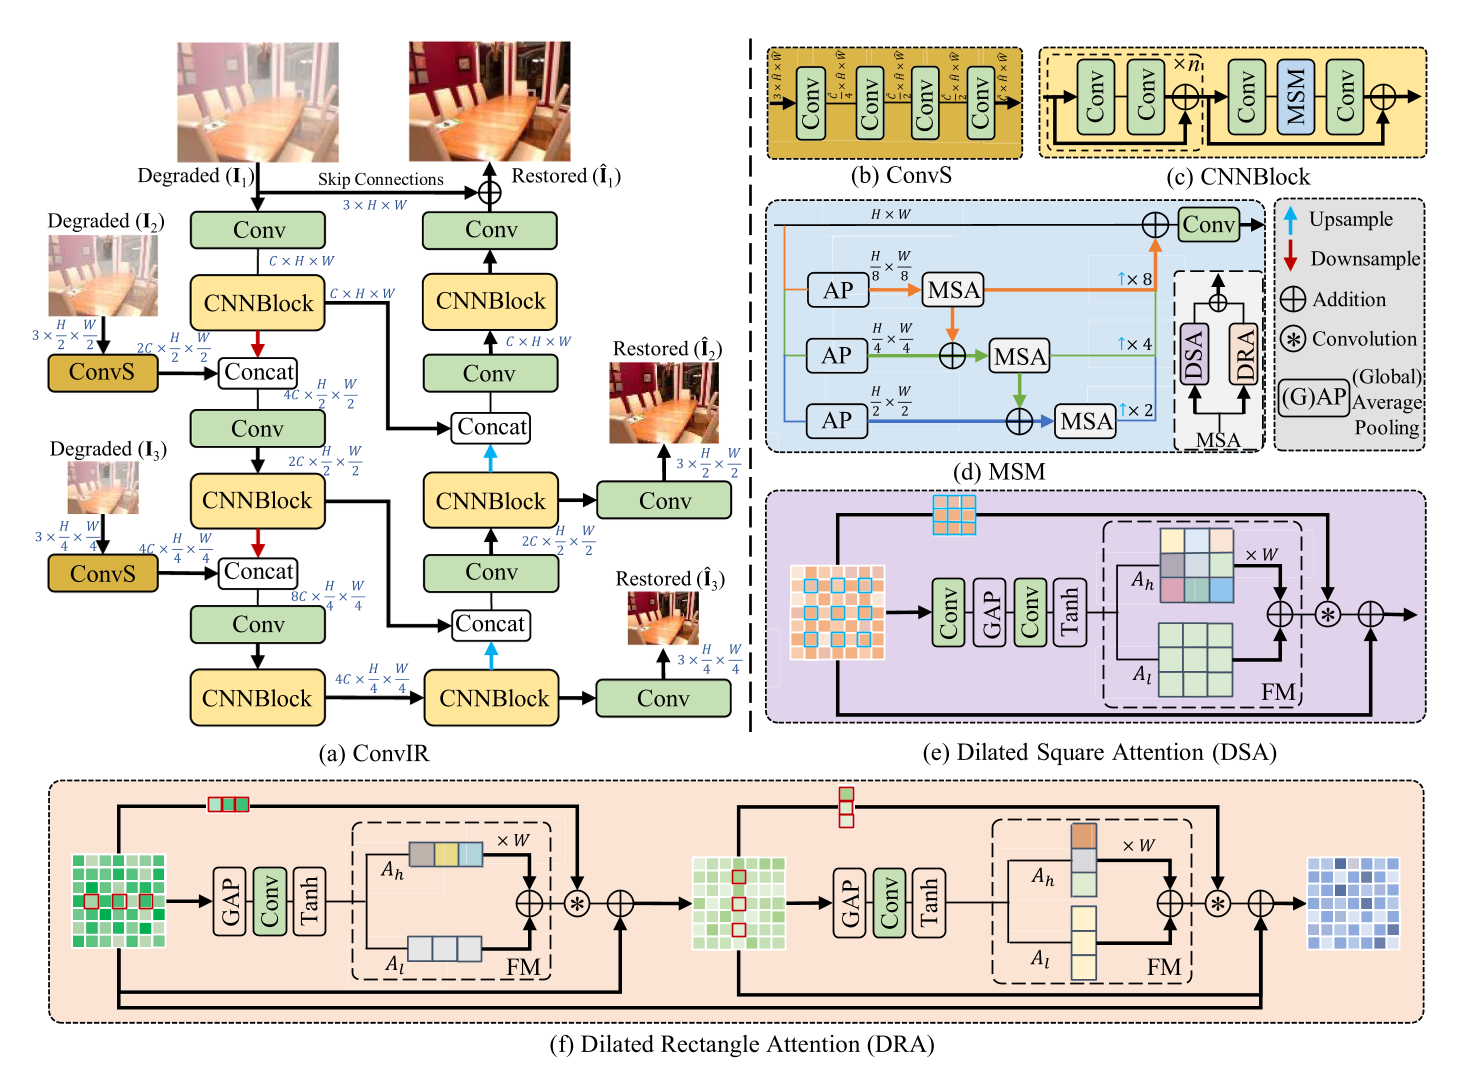
\includegraphics[width=\linewidth]{figures/architecture_complete.png}
  \caption{Schema generale dell'architettura completa (ConvIR)}
  \label{fig:architecture}
\end{figure*}

In figura~\ref{fig:architecture} è riportata l'architettura completa. La prima caratteristica interessante è che l'immagine in input viene elaborata non solo alla risoluzione primaria (256x256) generata dal dataloader,
ma viene ulteriormente sottocampionata (rispettivamente alla metà e a un quarto della risoluzione) e reinserita nella rete come input dei layer successivi.
L'obiettivo di questa configurazione multi-input multi-output è di analizzare l'immagine degradata secondo diversi livelli di dettaglio, e quindi di individuare pattern e feature più variegati e di diversa intensità.

L'encoder e il decoder hanno una struttura pressoché speculare, con tre skip connection che collegano i due rami, corrispondenti alle tre differenti risoluzioni a cui viene elaborata l'immagine. Come avviene di consueto nelle reti convolutive,
al ridursi della dimensione del tensore in larghezza e altezza, cresce il numero di canali. La feature extraction passa infatti attraverso i seguenti moduli:
\begin{enumerate}[label=\textbf{(\alph*)}]
  \item layer convolutivo semplice (blocco \textit{Conv} in verde in figura);
  \item \textit{ConvS}, blocco utilizzato solo per le versioni sottocampionate dell'immagine in input: consiste in una sequenza di quattro layer convolutivi che mantengono costanti le dimensioni di larghezza e altezza;
  \item \textit{CNNBlock}, blocco costituito da una serie di layer convolutivi raggruppati in \textit{n+1} blocchi residuali; nell'ultimo di questi blocchi viene inserito anche il \textit{MSM};
  \item \textit{MSM} (\textit{Multi-Scale Module}): fonde l'elaborazione di tre moduli \textit{MSA} (\textit{Multi-Scale Attention}), che operano appunto su tre scale dimensionali gradualmente decrescenti.
    Ogni \textit{MSA} combina di fatto l'output di un \textit{DSA} e un \textit{DRA};
  \item \textit{DSA} (\textit{Dilated Square Attention}): produce prima una attention map concentrandosi sulle aree quadrate del tensore in input, attraverso layer convolutivi e di pooling,
    e in seguito la elabora attraverso un filtro passa alto con parametri allenabili che sottrae unicamente la componente continua e tende ad esaltare quelle a più alta frequenza,
    tipicamente responsabili del blur;
  \item \textit{DRA} (\textit{Dilated Rectangle Attention}): modulo analogo al precedente ma focalizzato su pattern di forma rettangolare, combina attention map in senso verticale e orizzontale.
\end{enumerate}

L'architettura originale proposta in~\cite{convir} è stata utilizzata dagli autori in tre diversi formati: \textit{S (Small)}, \textit{B (Base)} e \textit{L (Large)}, ognuna caratterizzata da un numero variabile di blocchi residuali all'interno di ciascun modulo \textit{CNNBlock}.
Le configurazioni prevedevano \(n=3\), \(n=7\) e \(n=15\) rispettivamente per le varianti \textit{S}, \textit{B} e \textit{L}. La nostra scelta è ricaduta in una variante intermedia tra la \textit{S} e la \textit{B}, con \(\mathbf{n=6}\) blocchi residuali.
Abbiamo inoltre modificato il \textit{CNNBlock} rimuovendo completamente il modulo \textit{MSM} al suo interno. In questo modo, il training è risultato molto più rapido ed efficiente con solo una minima perdita di qualità del risultato finale.

La loss function utilizzata corrisponde alla somma pesata di un contributo calcolato nel dominio spaziale (\(\mathcal{L}_1\)) e uno in frequenza (\(\mathcal{L}_{freq}\)), in modo da considerare adeguatamente i diversi apporti dovuti alla presenza del blur:

\begin{align}
  \mathcal{L}_1 &= \mathcal{L}_{spatial} = \sum_{i=1}^{3}\frac{1}{P_i} \left\lVert \hat{\mathbf{I}}_i - \mathbf{Y}_i \right\rVert _1, \\
  \mathcal{L}_{freq} &= \sum_{i=1}^{3}\frac{1}{S_i} \left\lVert [\mathcal{R}(\hat{\mathbf{I}}_i), \mathcal{I}(\hat{\mathbf{I}}_i)] - [\mathcal{R}(\mathbf{Y}_i), \mathcal{I}(\mathbf{Y}_i)] \right\rVert _1,
\end{align}

Dove \(i\) indicizza gli output multipli a diverse risoluzioni; \(\hat{\mathbf{I}}\) e \(\mathbf{Y}\) rappresentano rispettivamente l'immagine elaborata dalla rete e il ground truth;
\(P\) e \(S\) indicano il numero totale di elementi dei tensori presi in considerazione, in modo da avere delle metriche normalizzate;
gli operatori \(\mathcal{R}()\) e \(\mathcal{I}()\) estraggono rispettivamente la parte reale e immaginaria della FFT operata sull'immagine.\\
La funzione di costo complessiva è così calcolata:

\begin{equation}
  \mathcal{L}_{tot} = \mathcal{L}_{spatial} + \lambda\mathcal{L}_{freq},
  \label{eq:total_loss_function}
\end{equation}

dove \(\lambda\) è un iperparametro impostato di default a \(0.01\).

\section{Observations}

Si illustrano di seguito le alterazioni apportate sull'architettura e processo di training, dettagliandone ragione e risultato.

\paragraph{Dataset}
I dataset usati sono principalmente due: GOPRO e RSBlur.
GOPRO è un dataset creato applicando un motion blur artificiale ai frame di una serie di video girate all'aperto, RSBlur invece usa una speciale fotocamera per creare contemporaneamente
una versione sfocata e una nitida della stessa immagine.

Per cercare di ottenere un risultato migliore possibile, abbiamo condotto dei test su entrambi i dataset che risultassero in una singola metrica che tenesse conto della performance su entrambi
i dataset, nello specifico:
\[ \text{Score} = \frac{1}{2}\sum_{i=1}^2 100 \cdot avg(\frac{PSNR_i}{33}, SSIM_i)\]
Dove $i$ indicizza il dataset su cui è stato svolto il test. Questa metrica è stata definita in modo da dare lo stesso peso alle metriche di SSIM e PSNR, oltre che ai due dataset: per ogni dataset si calcolano SSIM e PSNR medio, dopodichè si normalizza
il valore di PSNR in modo da riportarlo nell'intervallo [0, 1], si calcola la media tra PSNR e SSIM e la si moltiplica per 100, in modo da ottenere dei valori nell'intervallo [0, 100]; ottenuto questo valore quindi lo score è dato dalla media sui dataset.

Inizialmente il training è stato condotto usando GOPRO, ma dal punteggio è emerso come i modelli addestrati su RSBlur ottenessero una performance più bilanciata, mentre invece quelli addestrati su GOPRO tendevano a dare degli ottimi risultati sul test set, ma dei pessimi
risultati per quello che riguarda RSBlur. Nel corso dell'addestramento è stato provato come dataset anche un misto di RSBlur e GOPRO, con scarsi risultati, e alla fine si è deciso di usare esclusivamente RSBlur.

Il training set utilizzato consiste quindi in un sottoinsieme degli esempi di RSBlur, composto da 2500 immagini per il training set (di cui il 15\% è dedicato alla validazione) e 1000 per il test set. Sono stati prodotti diversi sottoinsiemi di RSBlur (con un numero di immagini
simile se non uguale a quelli citati in precedenza), compreso uno a risoluzione più bassa dell'originale, ottenuto tramite la funzione \texttt{resize(...)}\footnote{\url{https://docs.opencv.org/3.4/da/d54/group__imgproc__transform.html}} di OpenCV.
La versione finale consiste in un training set di 2755 esempi e un test set di 1000 esempi, ottenuto tramite crop delle immagini originale per riportare tutte le immagini alla stessa dimensione (invece che \texttt{resize} di OpenCV che interpola).

Oltre ai set citati, abbiamo anche usato un set di 32 immagini sfocate, senza versione nitida, scattato da noi, in modo da ottenere un riscontro più pratico e intuitivo (seppur non molto oggettivo). Nella sezione \ref{foto_esempio} si possono trovare i risultati su alcune di queste immagini.

\paragraph{Funzione di Training}
Ciascun Forward e Backward pass sono eseguiti, a fine di incrementare le prestazioni, con il formato floating point a 16 bit Brain Float,
sfruttando il meccanismo di troncamento automatico offerto da Pytorch chiamato \textit{AMP}\footnote{https://docs.pytorch.org/docs/stable/amp.html}.
Si nota che, in quanto in questo processo si vanno a perdere cifre decimali della mantissa, e dunque i contributi ai vari layer potrebbero risultare nulli,
la Loss viene scalata prima di applicare il backward pass con un $\mathrm{growth\_factor} = 2.0$

Alla funzione di costo descritta in precedenza (\ref{eq:total_loss_function}) abbiamo aggiunto un termine di gradient penalty, che appunto disincentivasse una crescita
eccessiva dei gradienti, consentendo quindi una regolarizzazione più efficace del modello. \\
Il backward pass comprende quindi un primo calcolo dei gradienti, secondo la loss function originale (\ref{eq:total_loss_function}), si ottiene poi la penalità,
accumulando la norma euclidea di tutti i gradienti appena ricavati, e la si somma alla funzione di costo precedente, infine vengono propagati i gradienti a partire da quest'ultima loss complessiva.

\paragraph{Iperparametri}

Di seguito gli iperparametri utilizzati assieme al valore selezionato a seguito di una esplorazione trial-and-error:
\begin{itemize}[topsep=0pt, noitemsep]
  \item \textbf{Batch Size}:
    \begin{itemize}[topsep=0pt, noitemsep]
      \item[\texttt{D}] Numero di Coppie di immagini, Example e Label, caricate in un ciclo di Stochastic Gradient Descent
      \item[\texttt{V}] \textbf{Valore}: $8$. Valori maggiori, eg. $12$ tendono a rallentare un ciclo di forward e backward propagation,
        mentre valori superiori o uguali a $32$ Esauriscono la
        memoria del GPU device utilizzato per i tests\footnote{RTX 3060, VRAM: 8GB}\\
    \end{itemize}

  \item
    \textbf{Optimizer}: L'ottimizzatore utilizzato \`e l'algoritmo di Adam con i seguenti parametri
    \begin{itemize}[topsep=0pt, noitemsep]
      \item[] $\beta_1 = 0.9$ peso del primo momento
      \item[] $\beta_2 = 0.999$ peso del secondo momento
    \end{itemize}

  \item
    \textbf{Learning Rate (Scheduling)}
    \begin{itemize}[topsep=0pt, noitemsep]
      \item[\texttt{D}] Moltiplicatore determinante Step Size dei parametri a partire dalla loss.
      \item[\texttt{V}] \textbf{Valore Iniziale}: $10^{-4}$. Circa la schedulazione, tra le strategie di schedulazione considerate,
        in particolare, \textit{Momentum}, \textit{Warmup}, \textit{Decay}, sono state impiegate la strategia di \textit{Gradual Warmup}
        per le prime $N - 3$ epoche, seguita da un \textit{Cosine Decay} nelle
        epoche rimanenti. Si nota che \`e stato evitato l'impiego del momento in quanto superfluo con ottimizzatori a learning
        rate adattivo.\footnote{Infatti, il calcolo del momento \`e incluso nell'Adam Optimizer}
    \end{itemize}

  \item
    \textbf{Weight Decay}:
    \begin{itemize}[topsep=0pt, noitemsep]
      \item[\texttt{D}] Nell'ambito dell'ottimizzatore Adam implementato da Pytorch, fattore moltiplicativo dei componenti del gradiente da
        ogni layer.  Quando \`e diverso da zero, ciascun componente \`e moltiplicato per $1 + \mathrm{weight\_decay}$
      \item[\texttt{V}] $0$
    \end{itemize}

  \item
    \textbf{Accumulate Gradient Frequency}:
    \begin{itemize}[topsep=0pt, noitemsep]
      \item[\texttt{D}] Frequenza, in termini di numero di batches processati, di applicazione dei gradienti calcolati dagli ultimi
        $\mathrm{agf}$ backward passes
      \item[\texttt{V}] $1$. Valori Maggiori tendono a rendere La curva della Loss instabile
    \end{itemize}

  \item
    \textbf{$\lambda$}:
    \begin{itemize}[topsep=0pt, noitemsep]
      \item[\texttt{D}] Fattore di peso del contributo della Loss nel dominio di Fourier
      \item[\texttt{V}] $0.1$
    \end{itemize}

  \item
    \textbf{Image Distance Metric}:
    \begin{itemize}[topsep=0pt, noitemsep]
      \item[\texttt{D}] Funzione utilizzata per comparare una coppia di immagini nel calcolo della Loss.
      \item[\texttt{V}] Norma L1 della differenza (invariata rispetto all'architettura di riferimeento)
    \end{itemize}
\end{itemize}

\paragraph{Data Augmentation}

Seguendo il codice originale, abbiamo mantenuto pressoché invariate le trasformazioni usate dagli autori per la data augmentation, ovvero:
\begin{itemize}
  \item \texttt{RandomCrop(256)}: Estrae un crop quadrato di lato 256 pixel, rendendo il training estremamente più veloce
  \item \texttt{RandomHorizontalFlip(p=0.5)}: Decide casualmente (con una probabilità del 50\%) se ruotare intorno all'asse verticale il crop ottenuto al passo precedente
  \item \texttt{ToDtype(torch.get\_default\_dtype())}: Cast degli elementi del tensore a \texttt{torch.float32}
  \item \texttt{NormalizeRange()}: Normalizza i valori del tensore nell'intervallo [0, 1]
\end{itemize}

Queste trasformazioni sono volte ad aumentare artificialmente la dimensione del dataset, senza però andare ad alterare l'informazione associata al blur: inizialmente abbiamo provato altre trasformazioni come ad esempio
\texttt{ColorJitter}, ma è risultato evidente che

\paragraph{Alterazioni sull'Architettura}

\section{Results}

\begin{figure*}[t]
  \begin{mdframed}[
      linewidth=1pt,
      innertopmargin=6pt,
      innerbottommargin=6pt,
      innerleftmargin=6pt,
      innerrightmargin=6pt
      linecolor=black,
      nobreak
    ]

    \centering
    \subfloat[boh]{
      \centering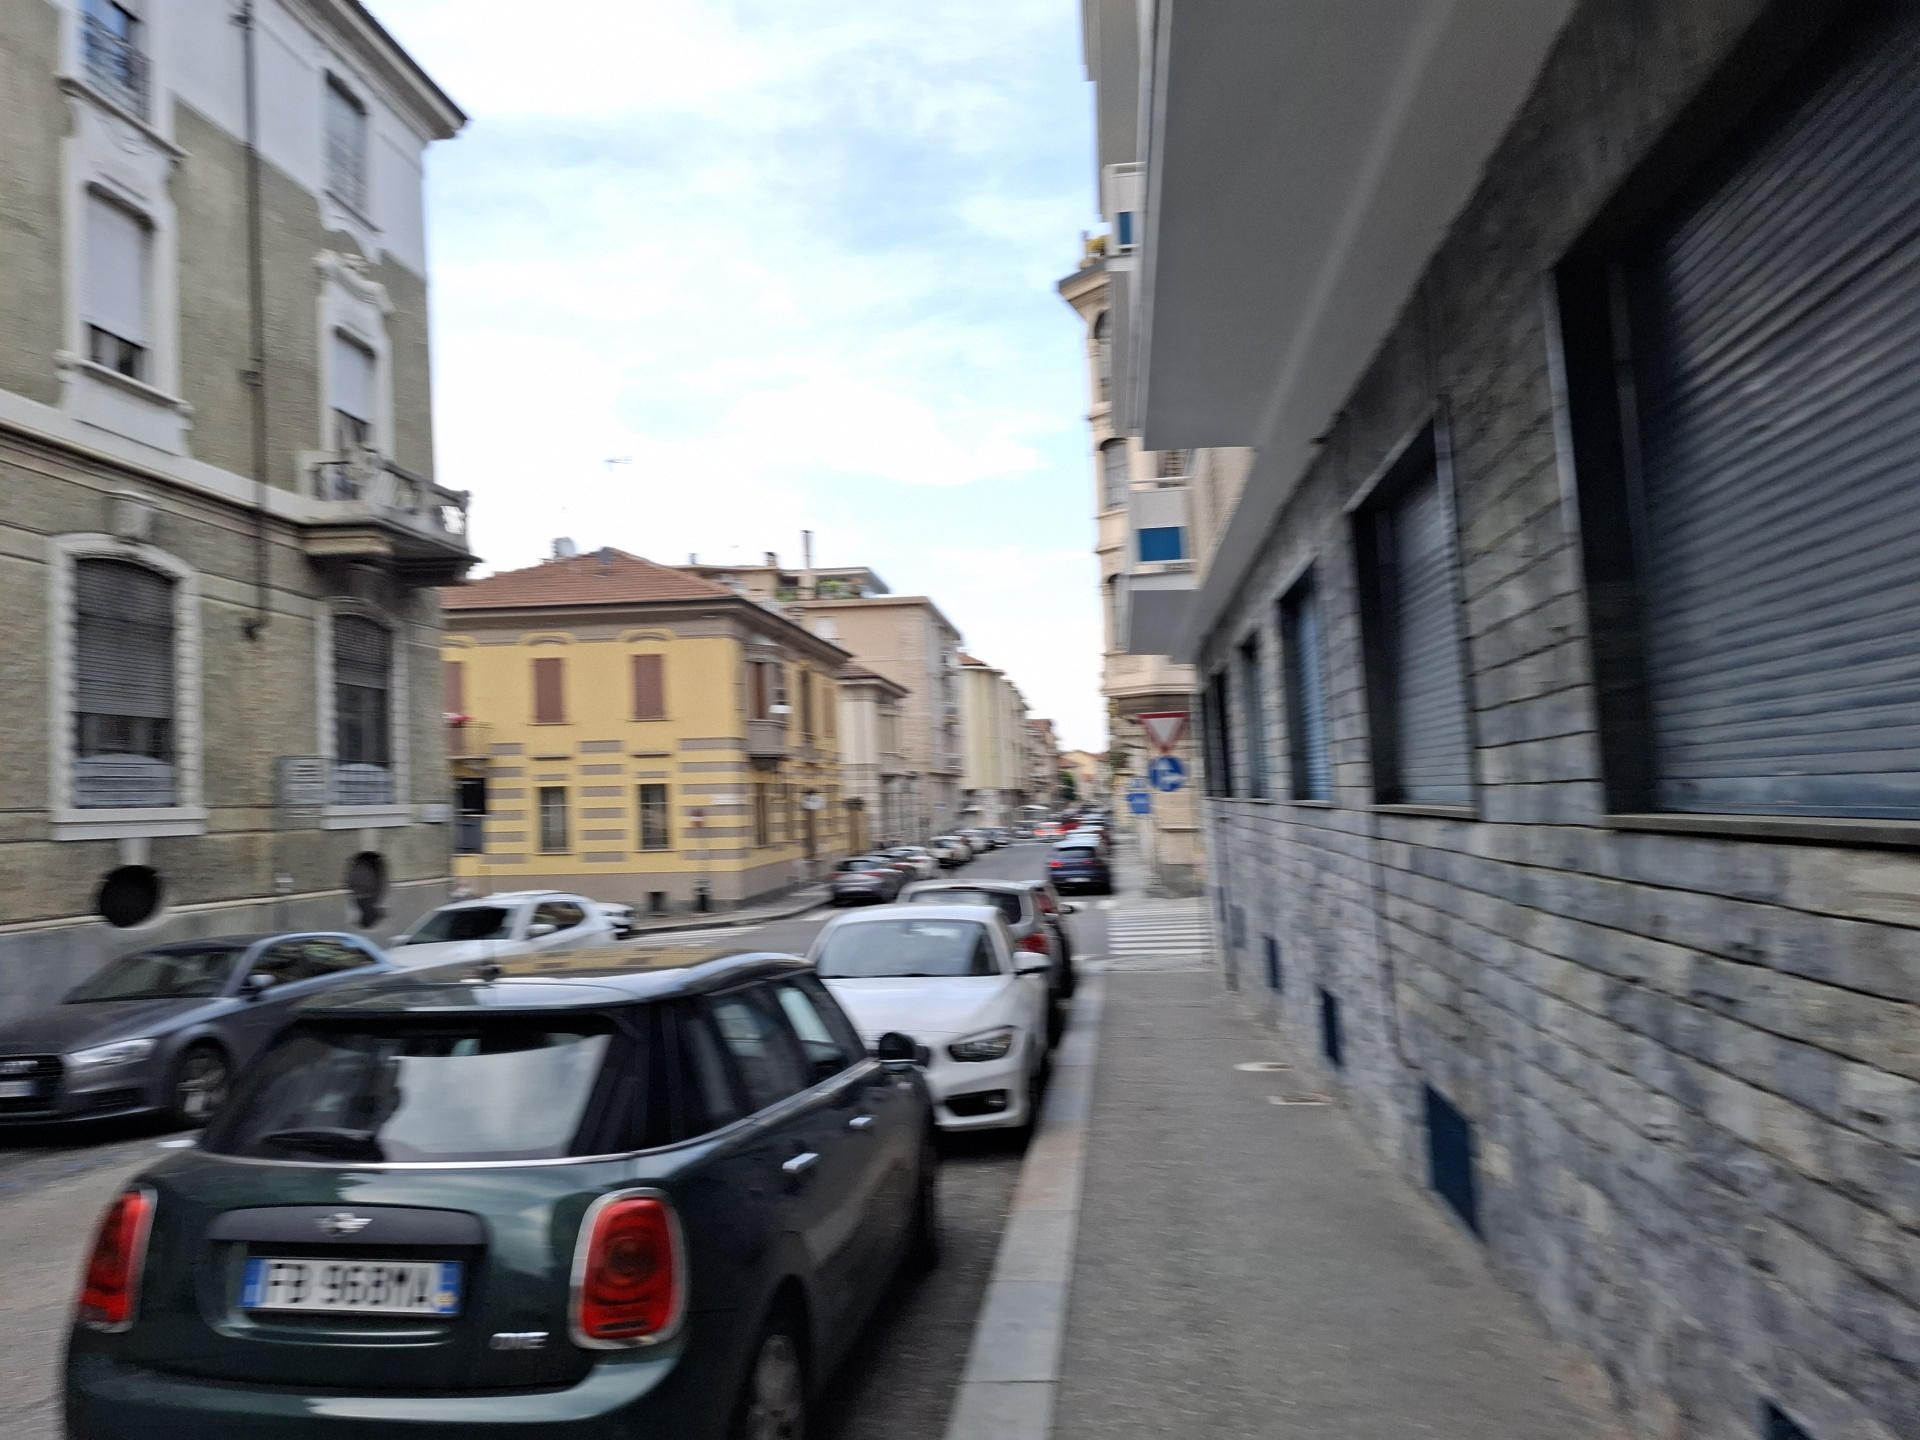
\includegraphics[width=0.31\linewidth]{figures/sample_imgs/20250503_184657.jpg}
    }\hspace{0.1cm}\hfill
    \subfloat[boh]{
      \centering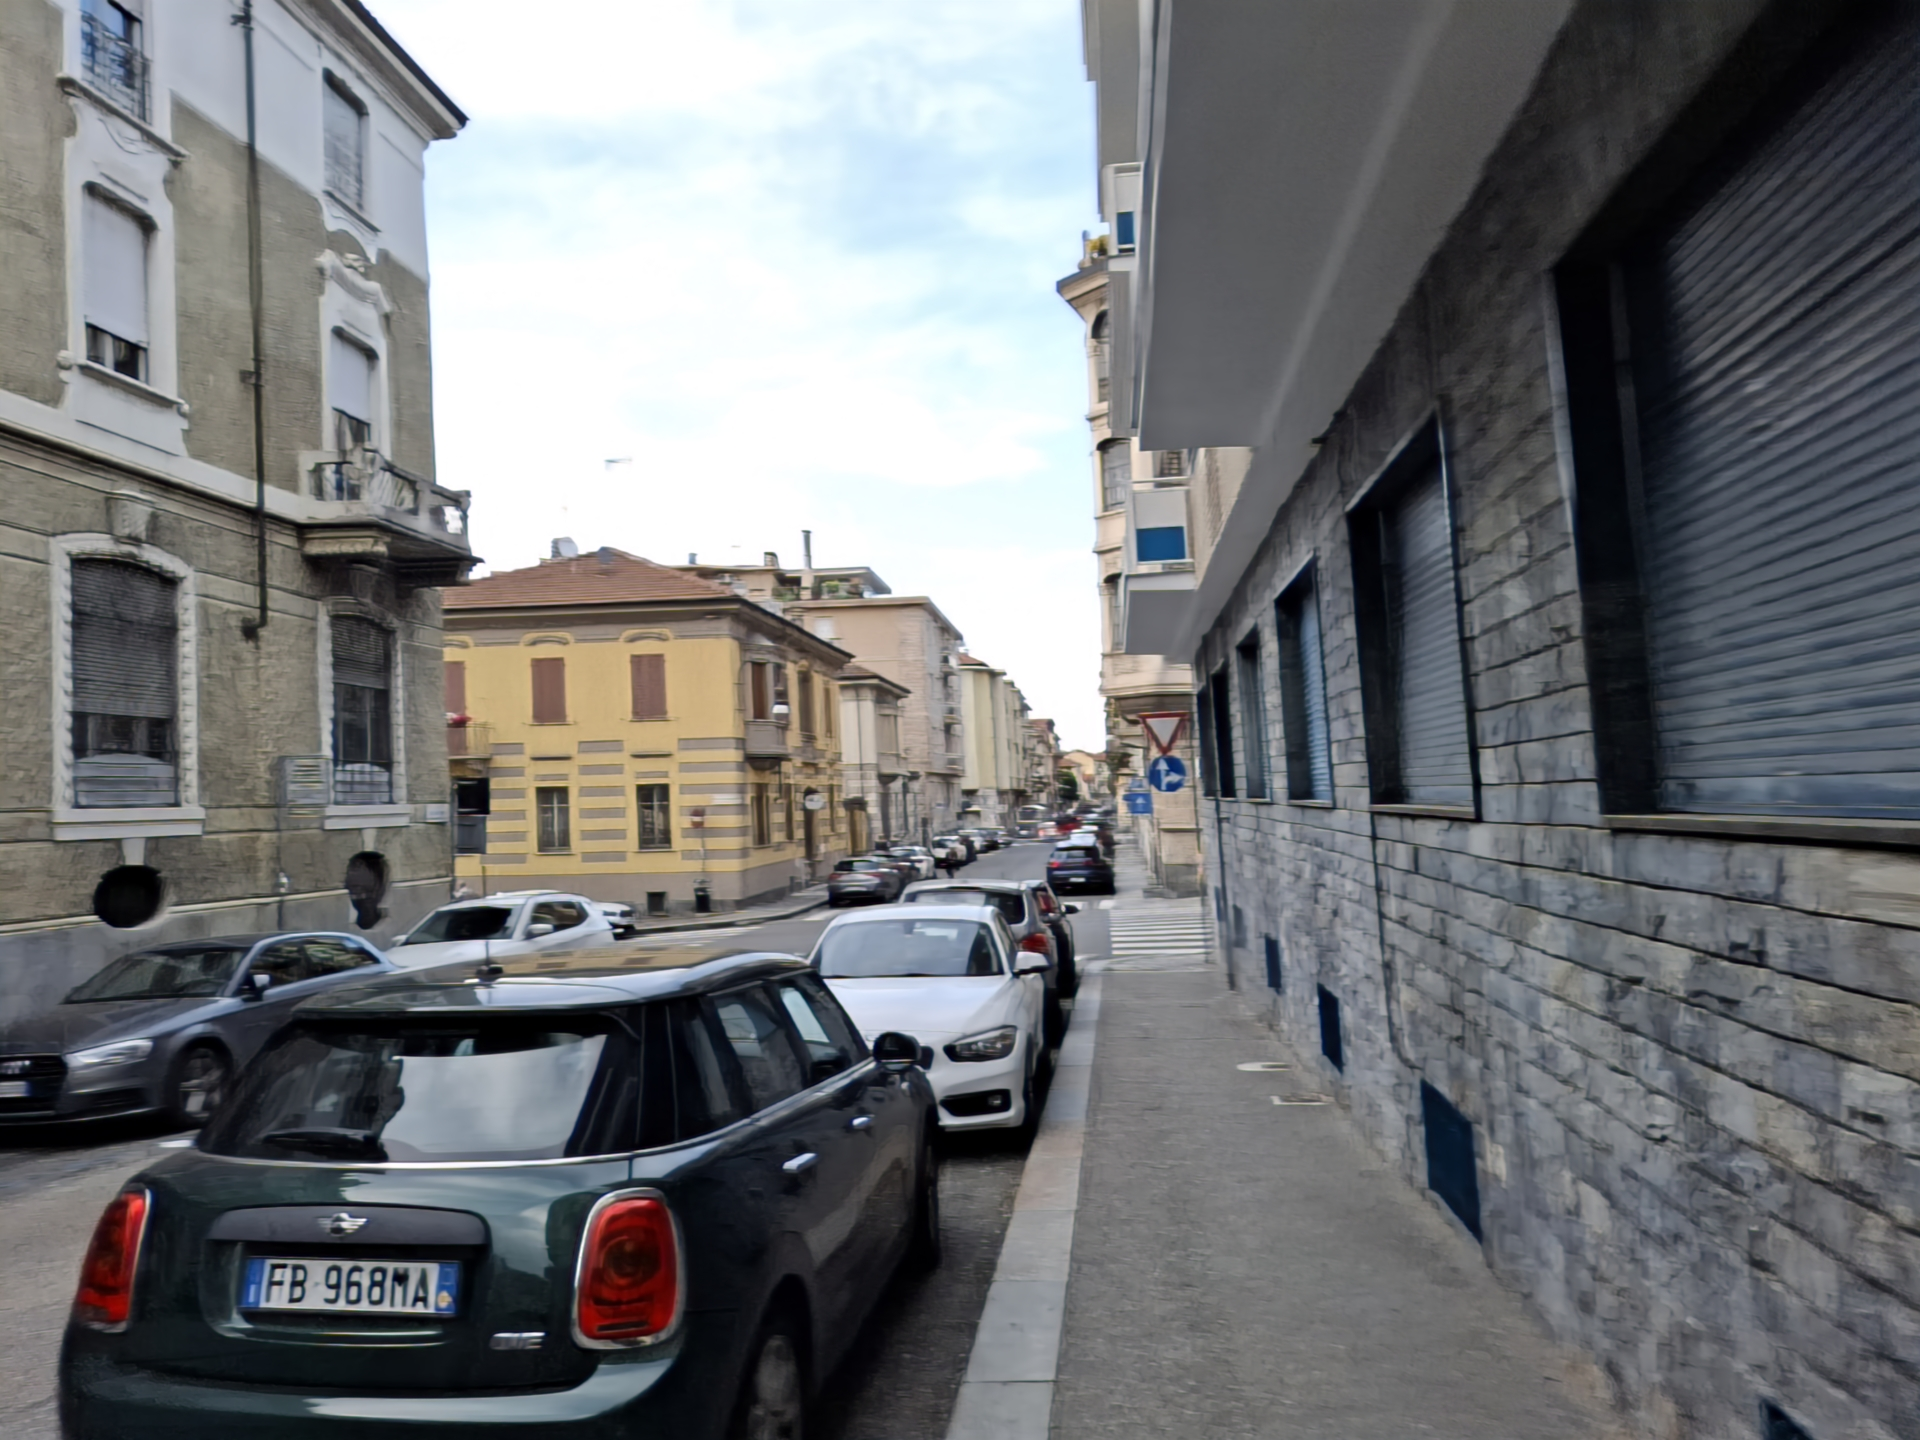
\includegraphics[width=0.31\linewidth]{figures/sample_imgs/20250503_184657_deblurred.jpg}
    }\hspace{0.1cm}\hfill
    \subfloat[boh]{
      \centering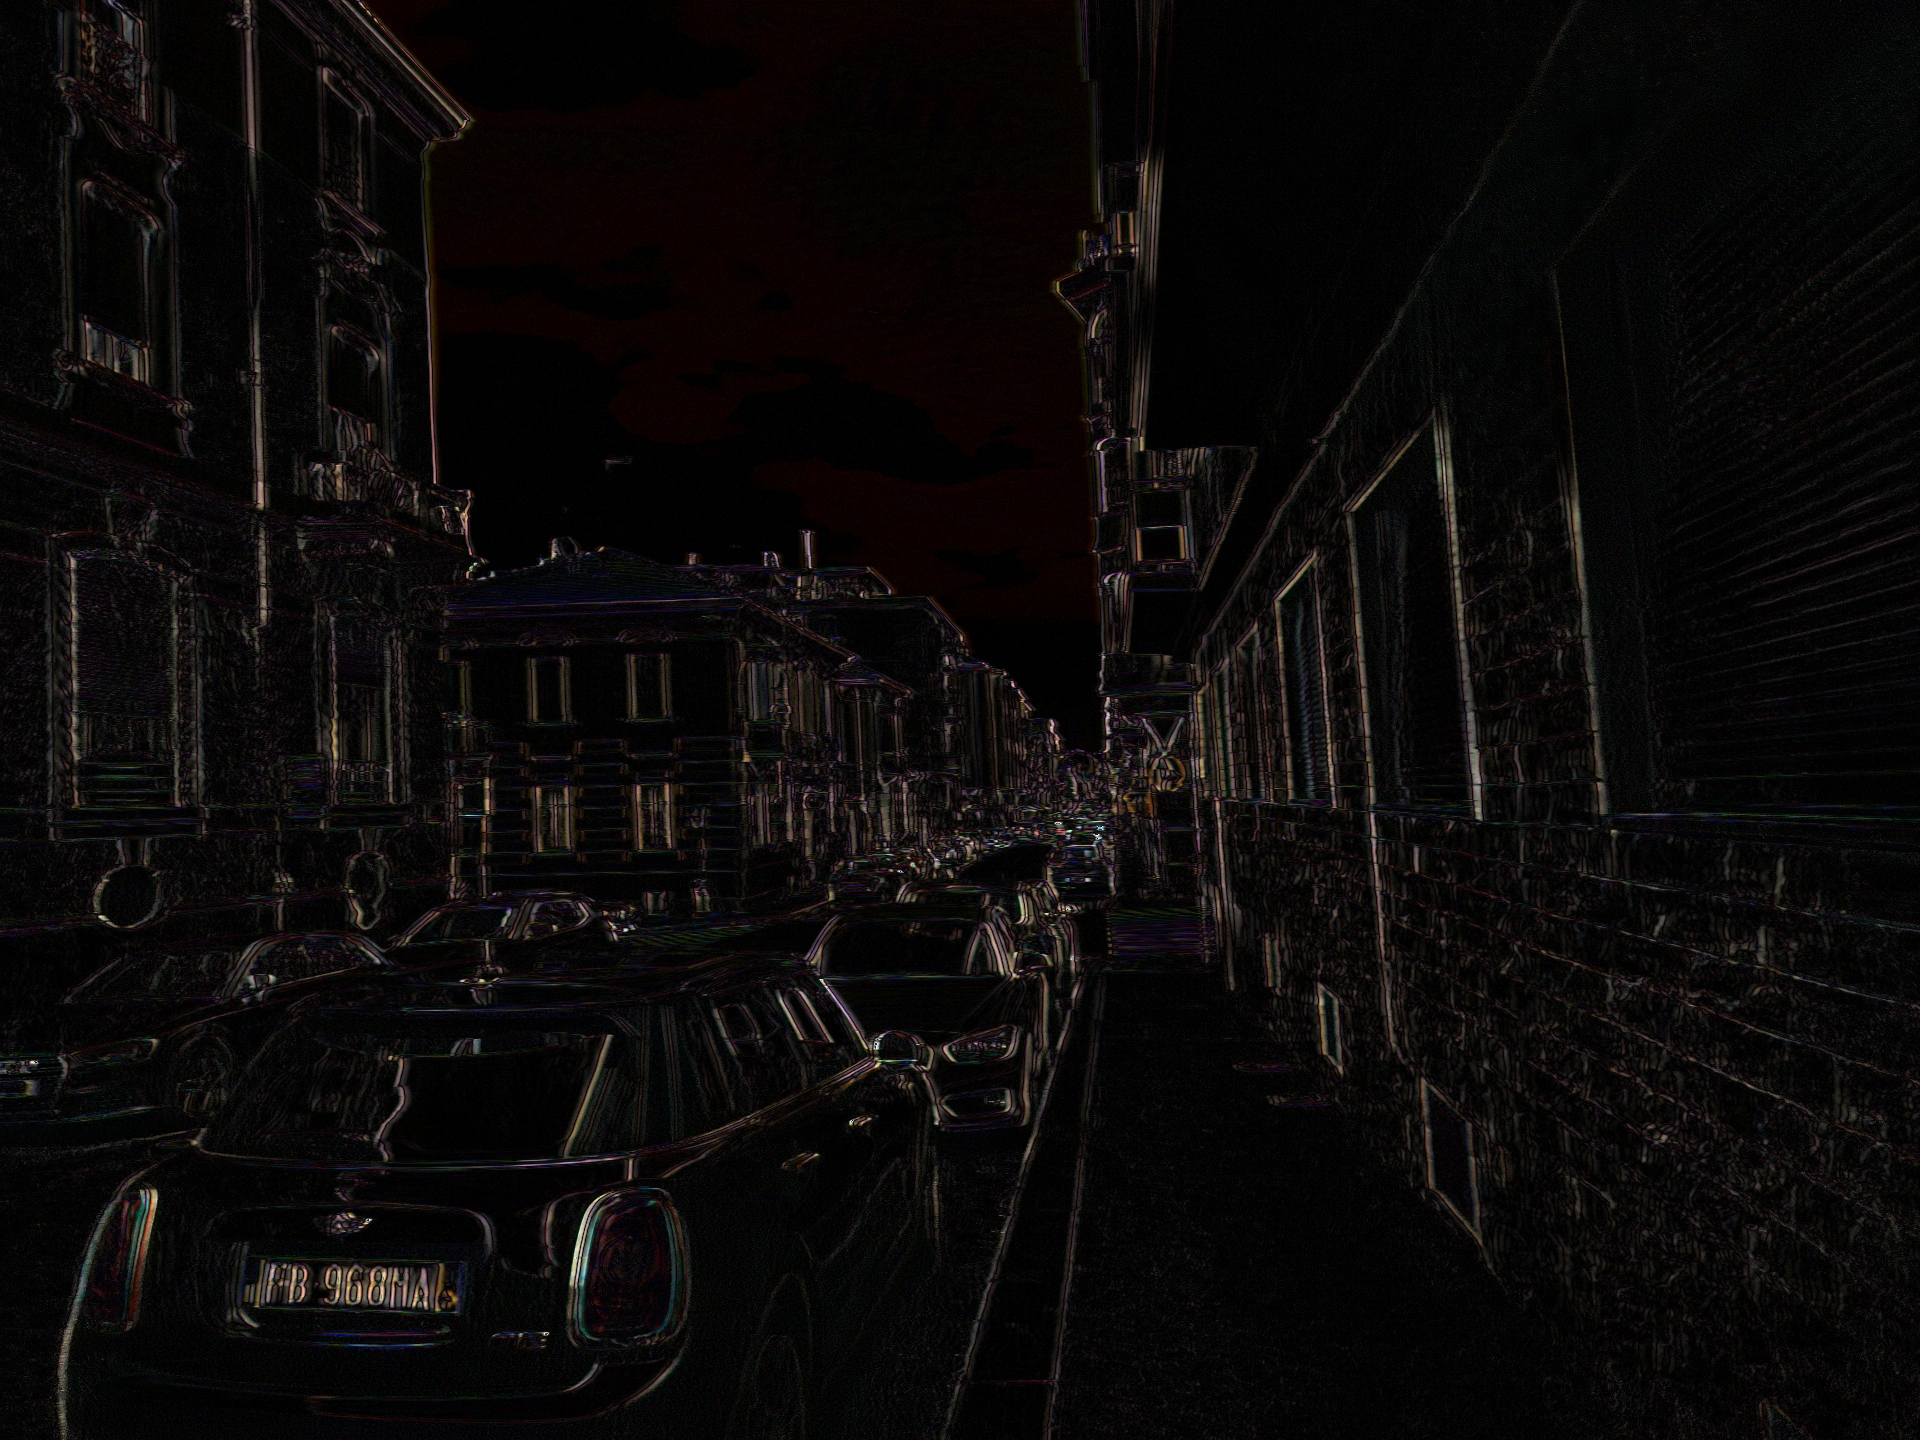
\includegraphics[width=0.31\linewidth]{figures/sample_imgs/comparison_20250503_184657.jpg}
    }\hspace{0.1cm}\hfill
    \\
    \subfloat[boh]{
      \centering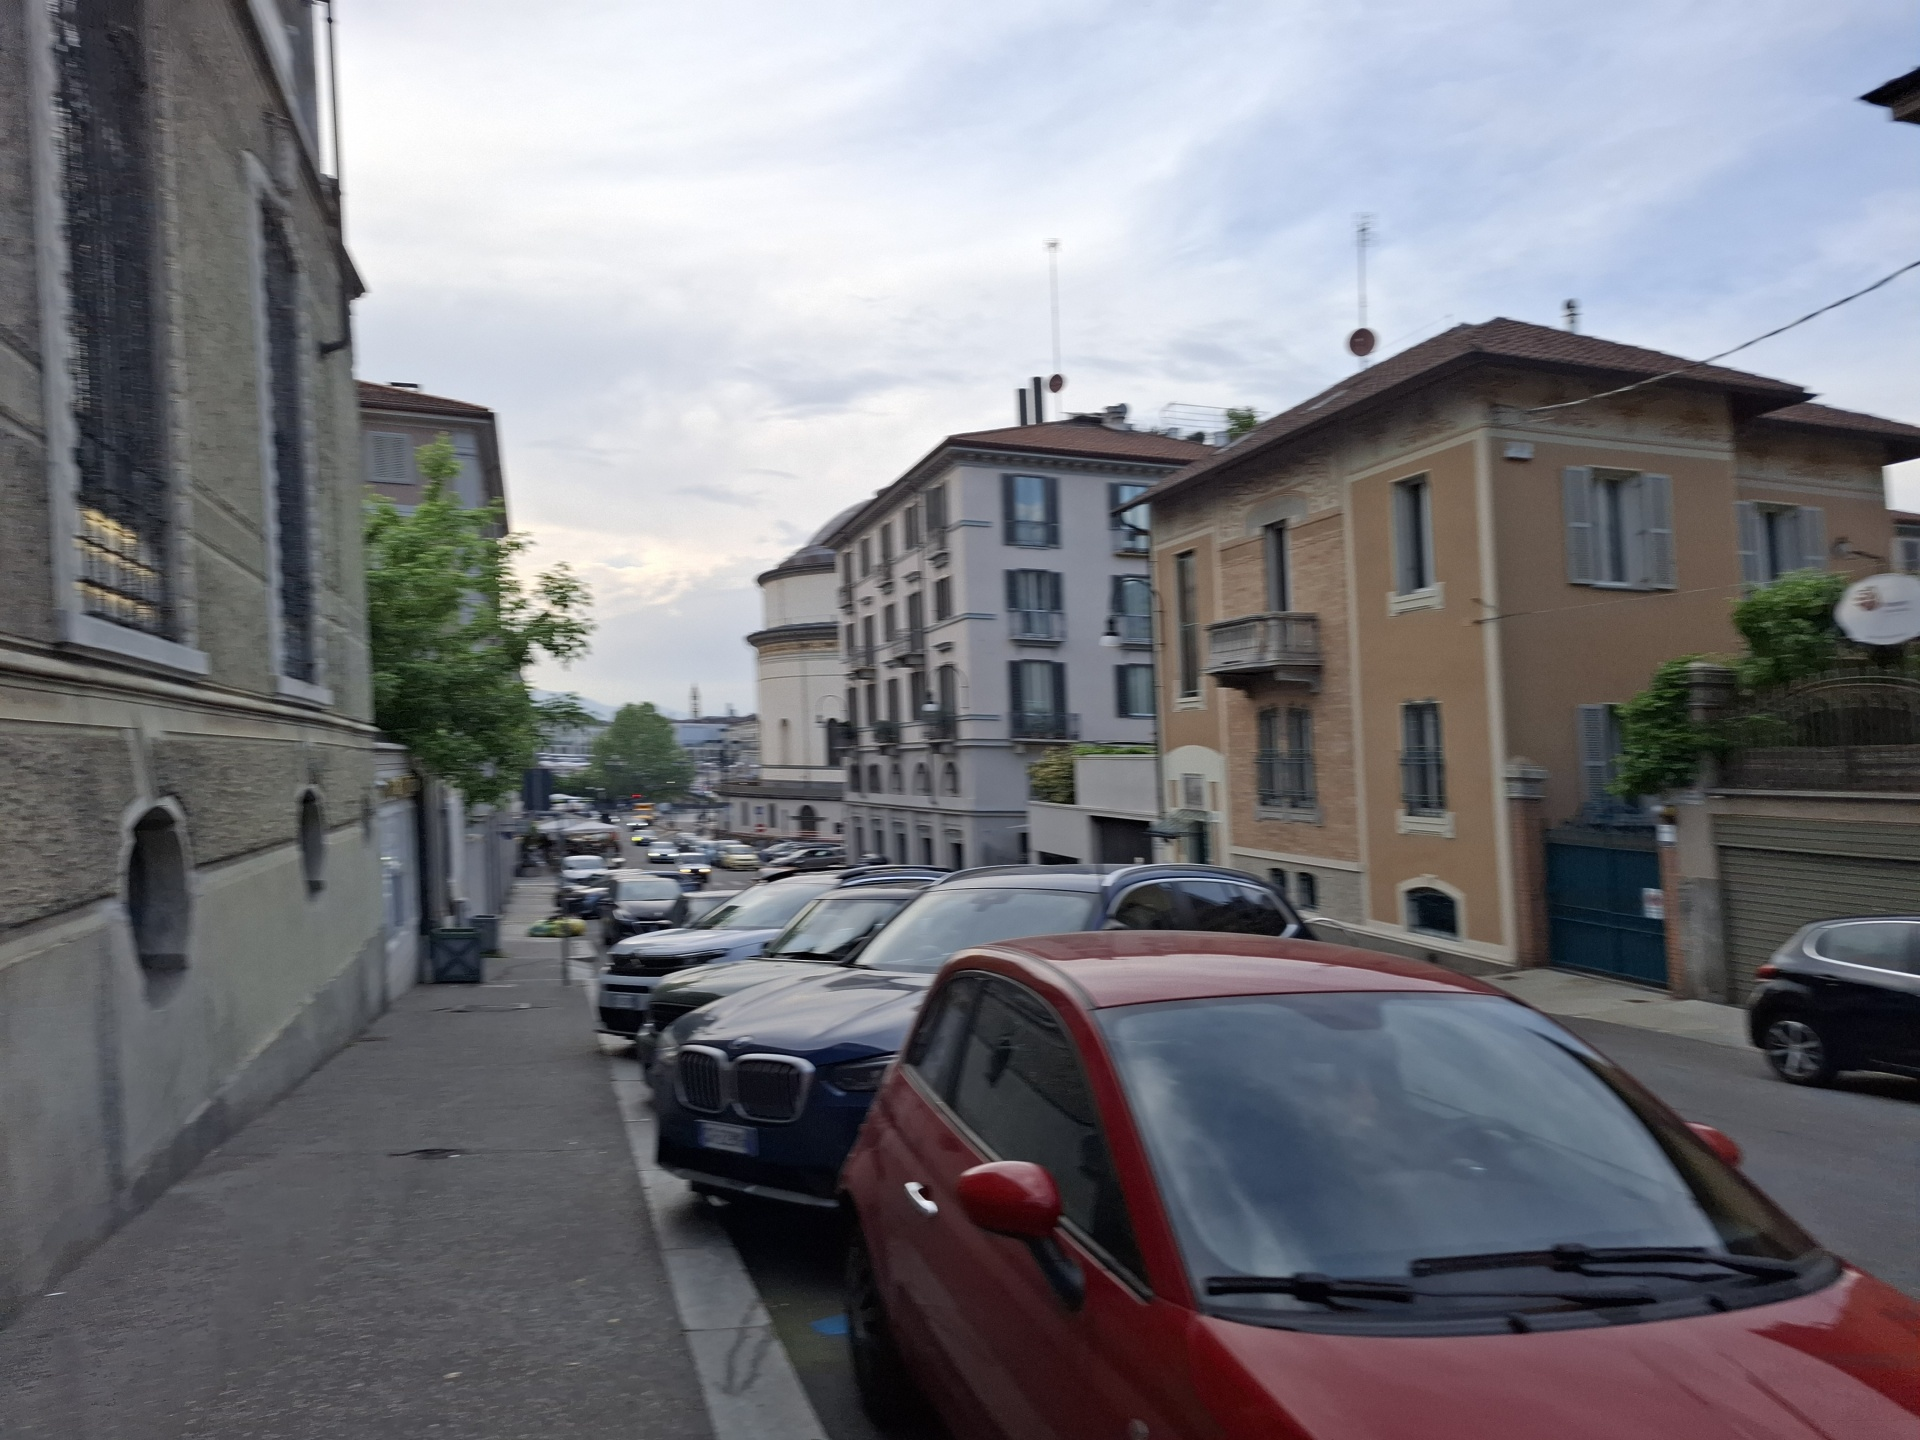
\includegraphics[width=0.31\linewidth]{figures/sample_imgs/20250503_184720.jpg}
    }\hspace{0.1cm}\hfill
    \subfloat[boh]{
      \centering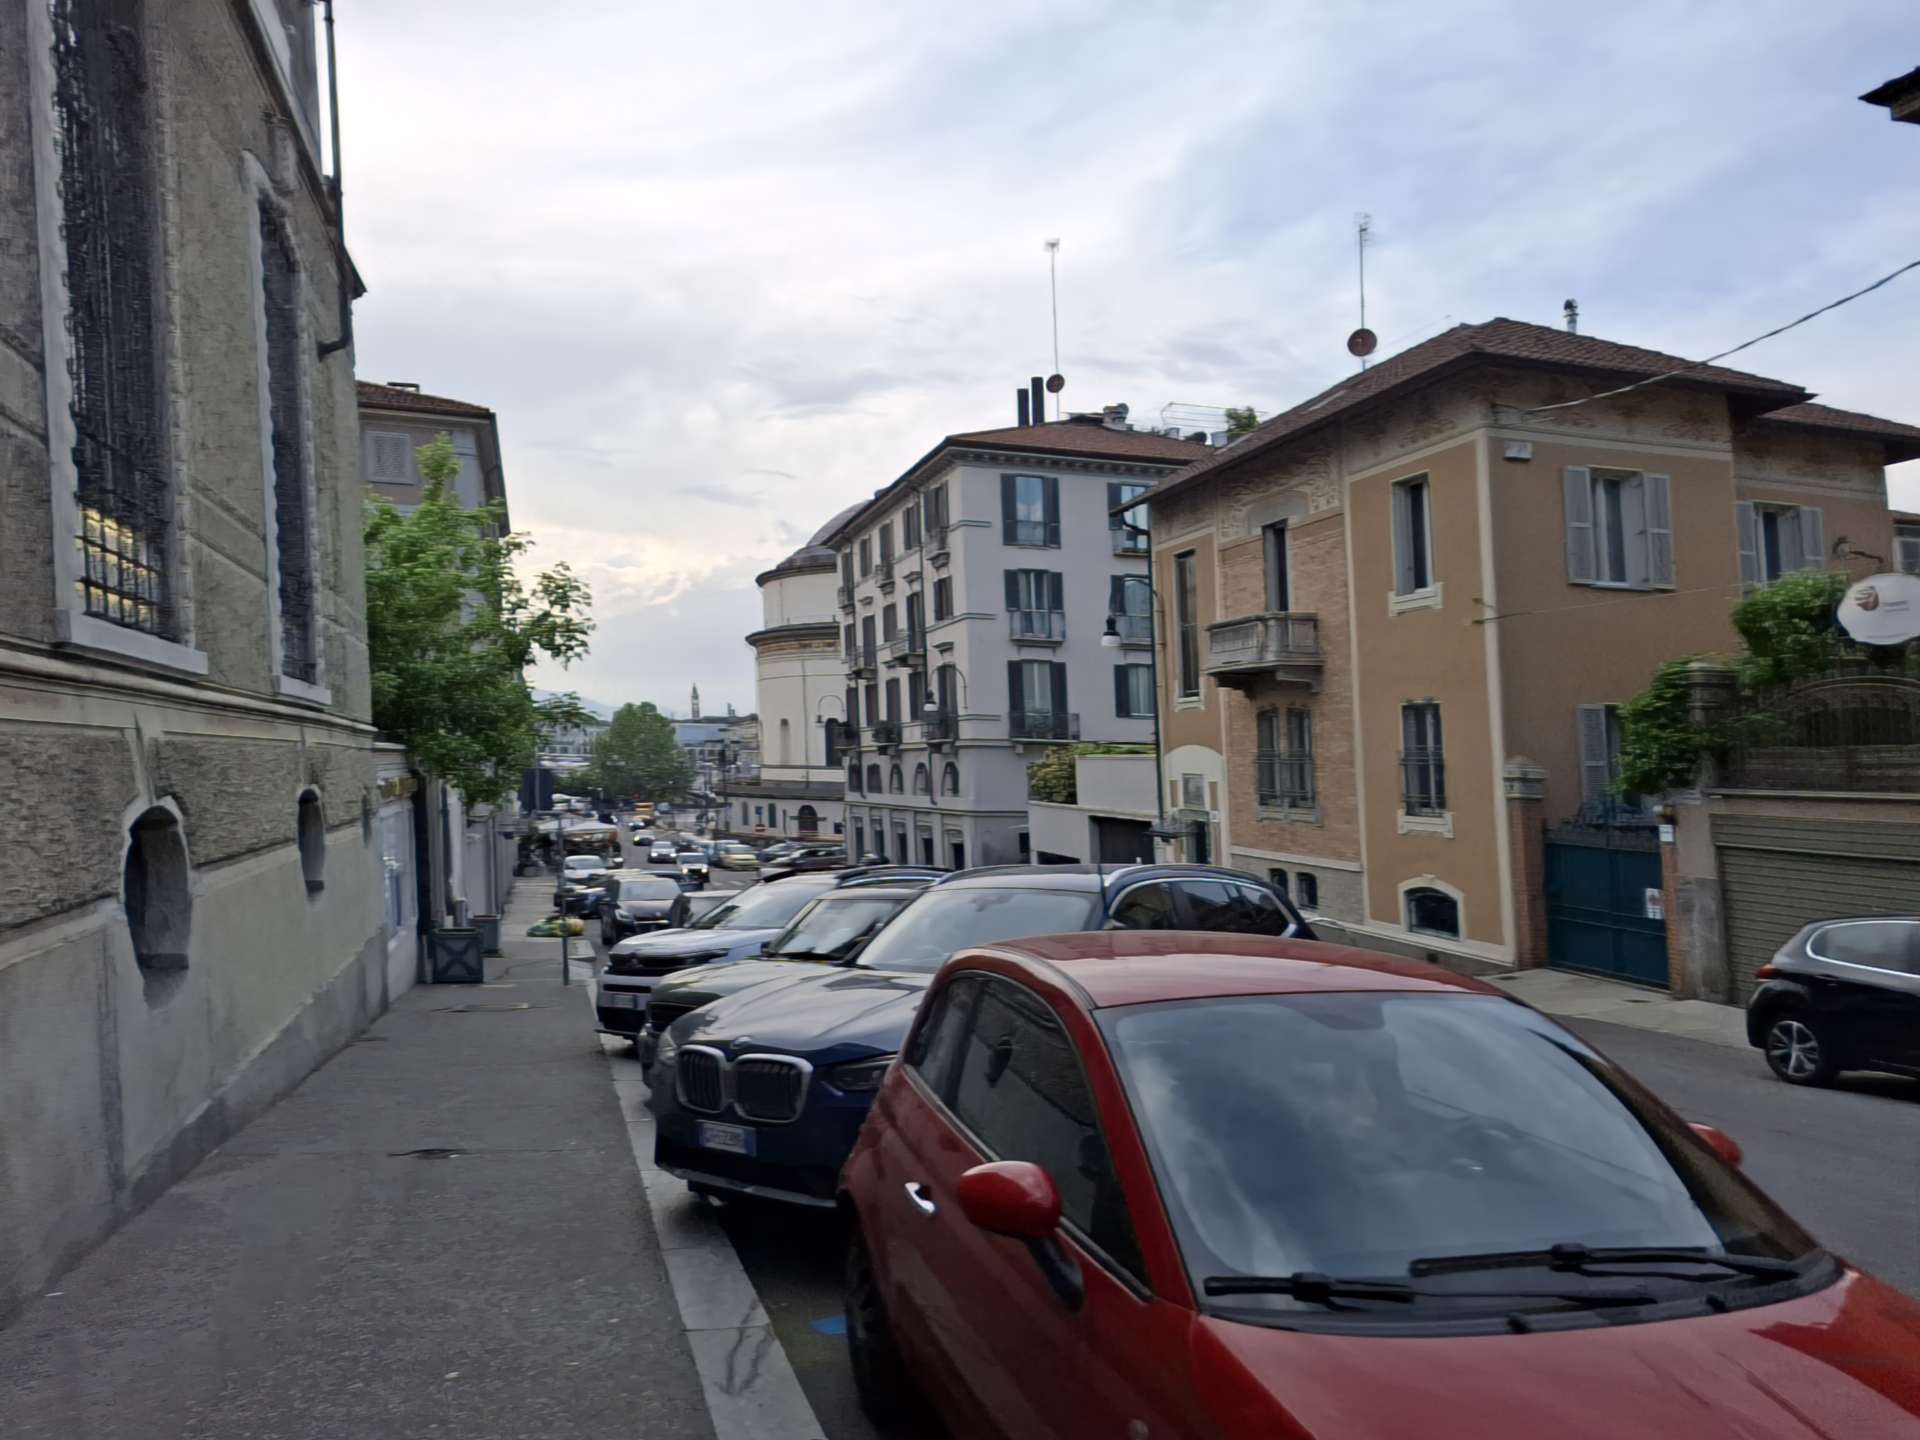
\includegraphics[width=0.31\linewidth]{figures/sample_imgs/20250503_184720_deblurred.jpg}
    }\hspace{0.1cm}\hfill
    \subfloat[boh]{
      \centering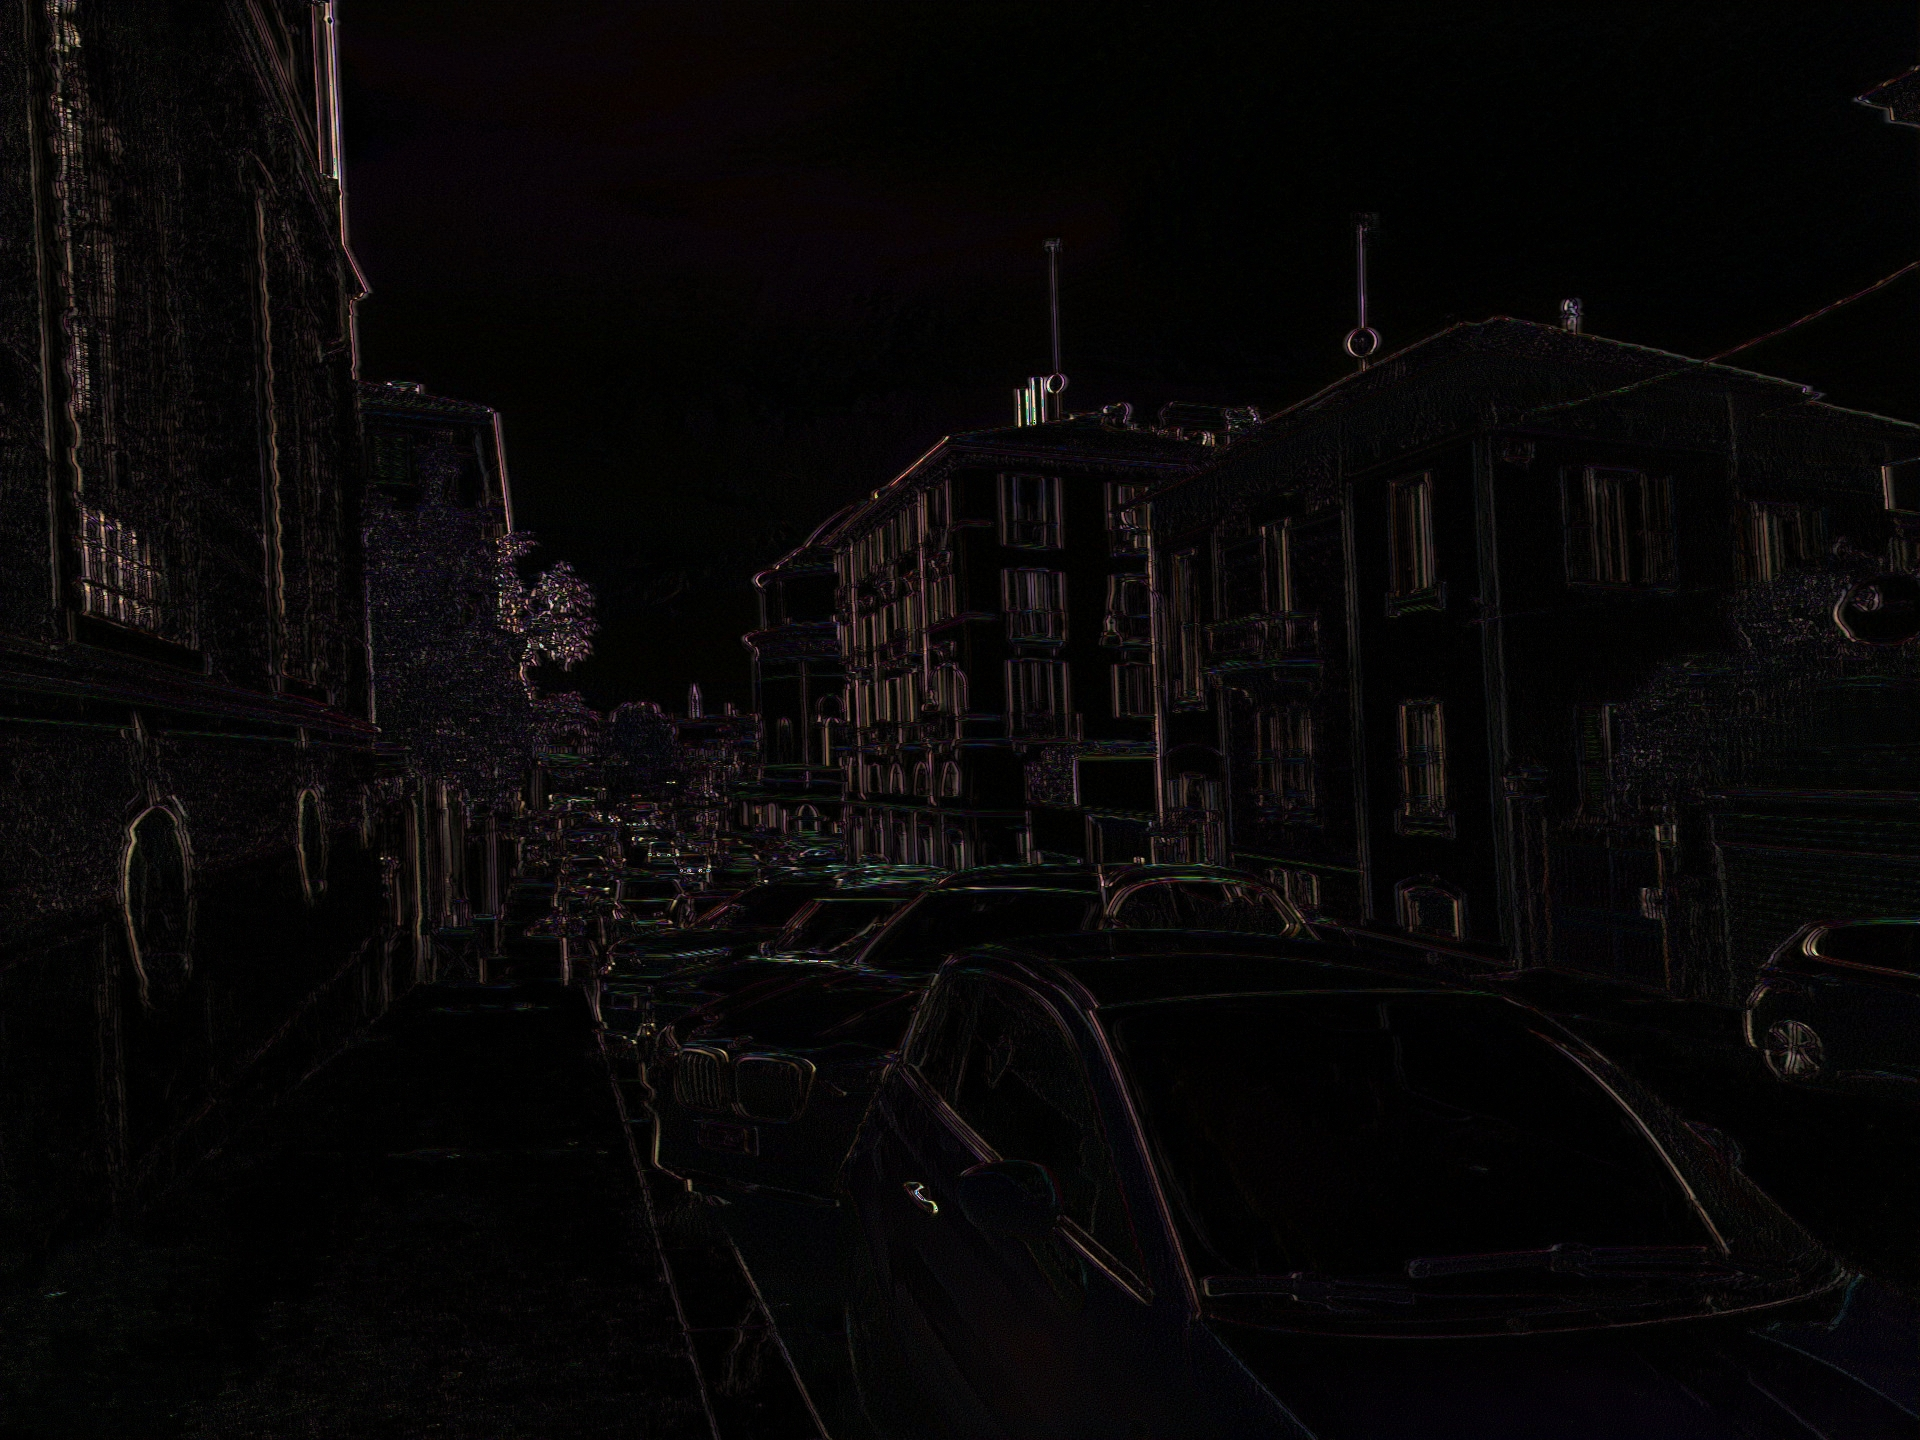
\includegraphics[width=0.31\linewidth]{figures/sample_imgs/comparison_20250503_184720.jpg}
    }\hspace{0.1cm}\hfill
    \\
    \subfloat[boh]{
      \centering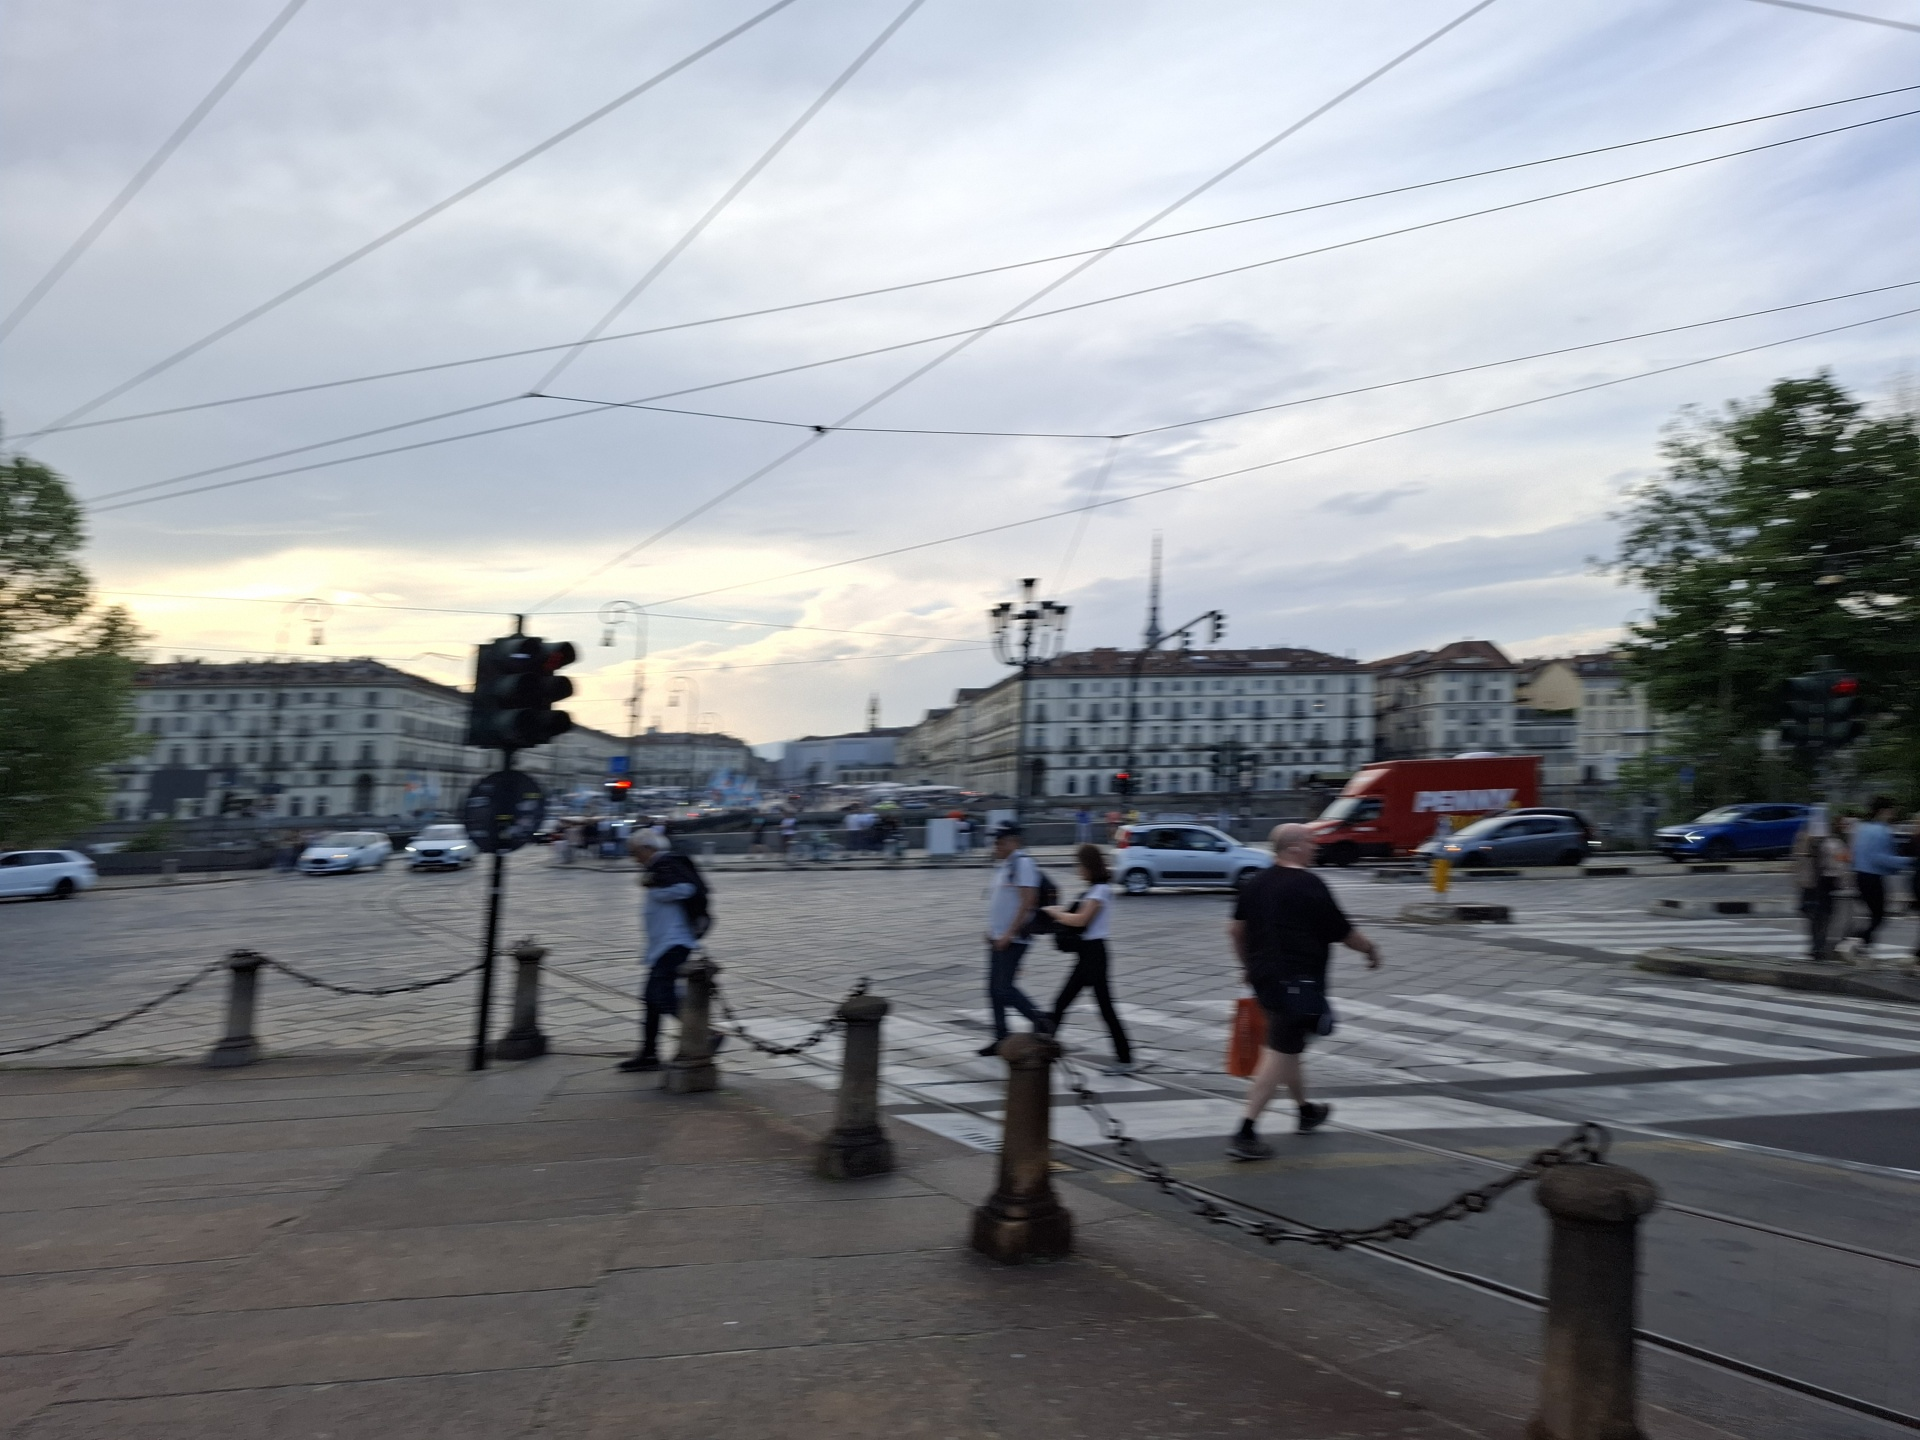
\includegraphics[width=0.31\linewidth]{figures/sample_imgs/20250503_185104.jpg}
    }\hspace{0.1cm}\hfill
    \subfloat[boh]{
      \centering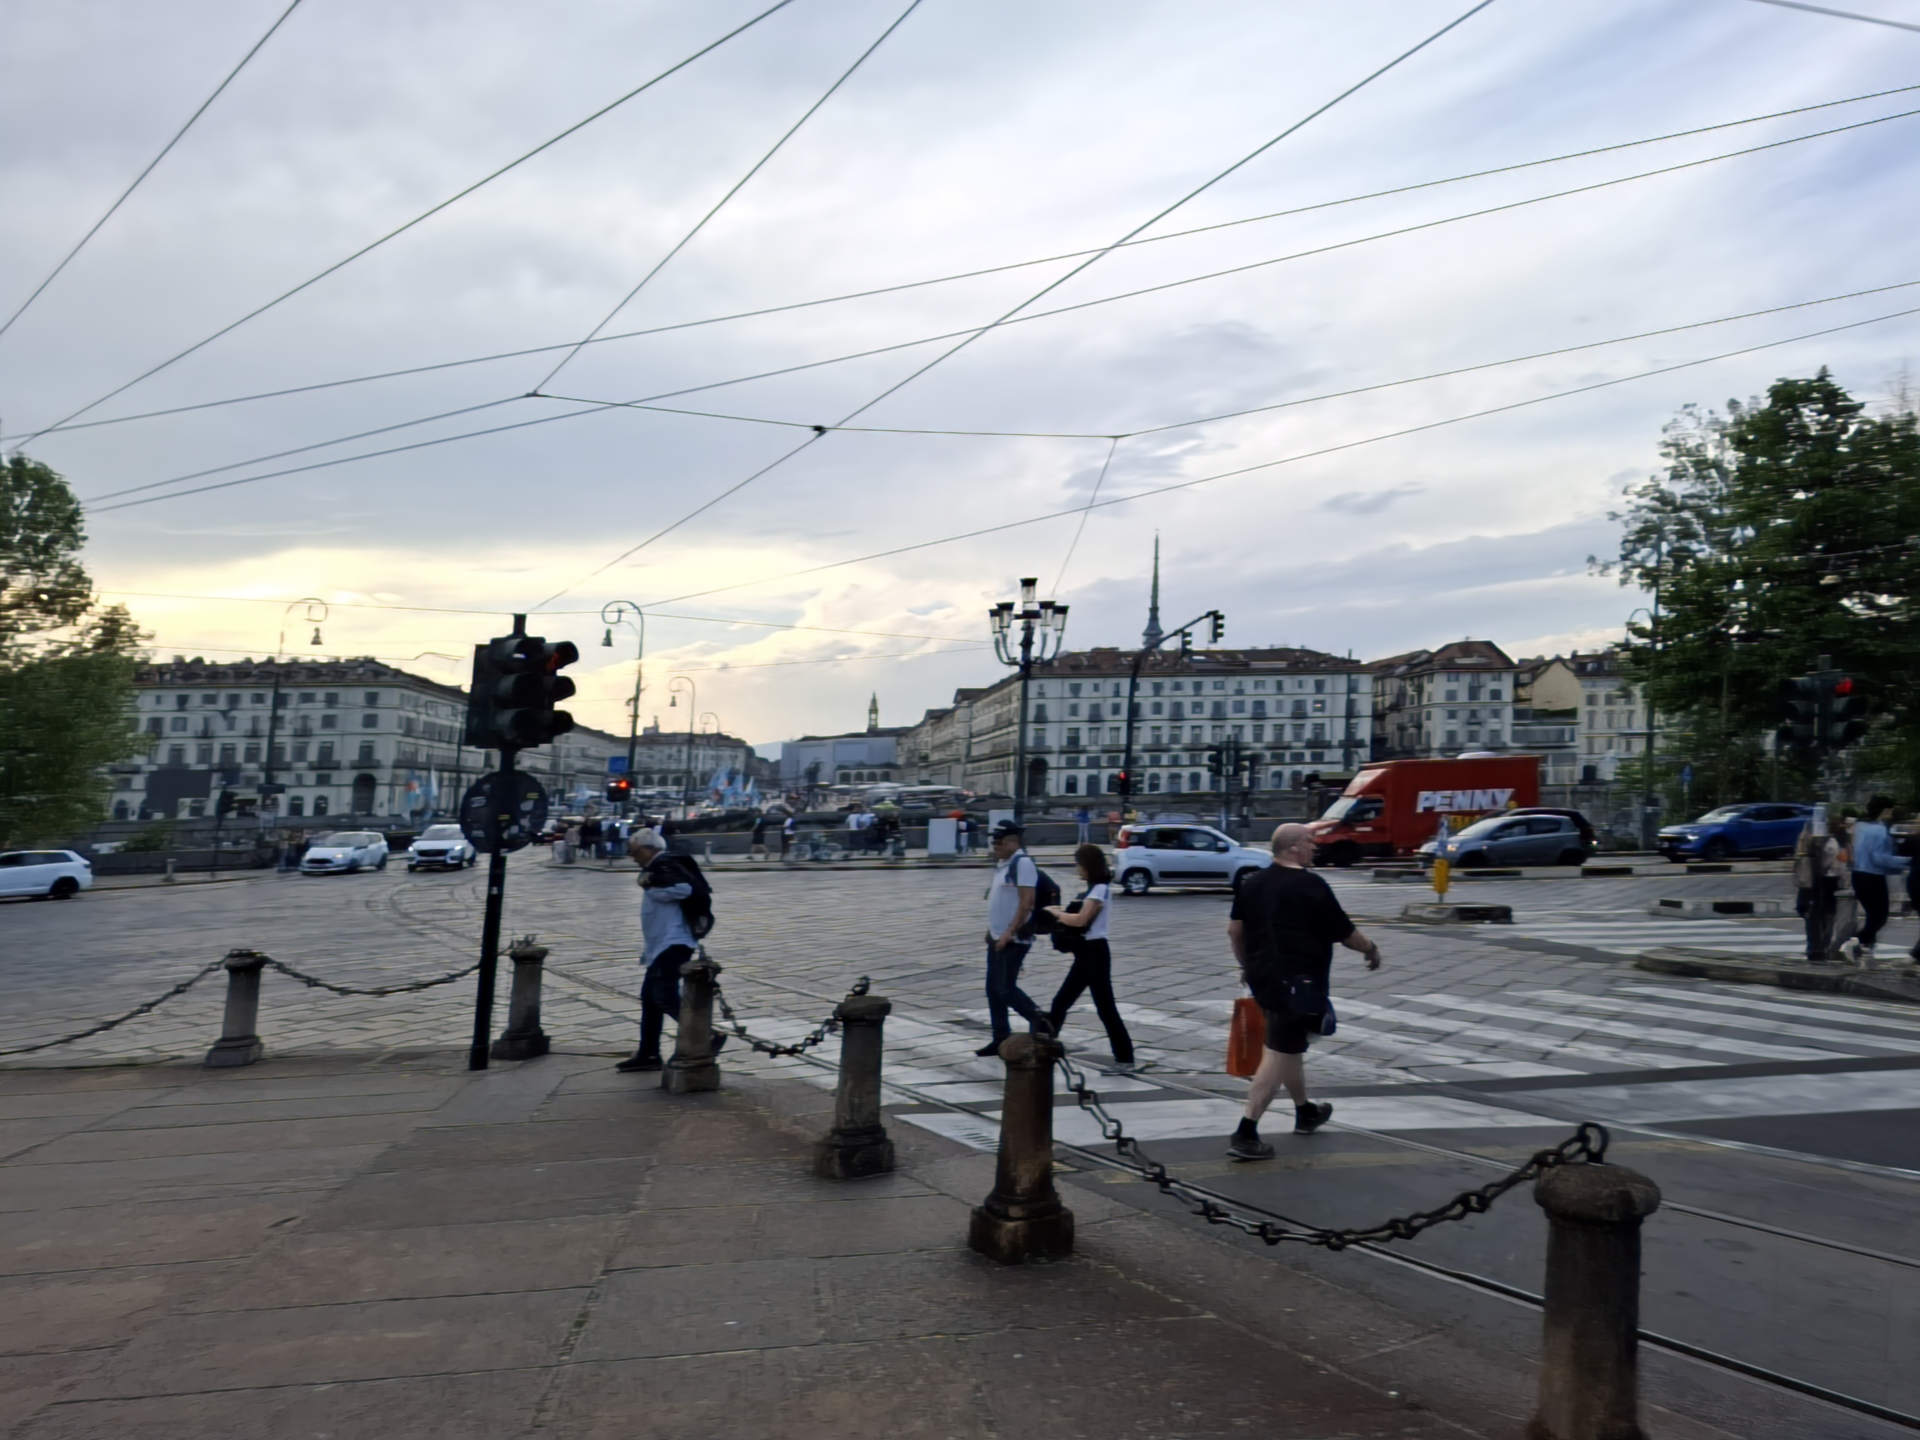
\includegraphics[width=0.31\linewidth]{figures/sample_imgs/20250503_185104_deblurred.jpg}
    }\hspace{0.1cm}\hfill
    \subfloat[boh]{
      \centering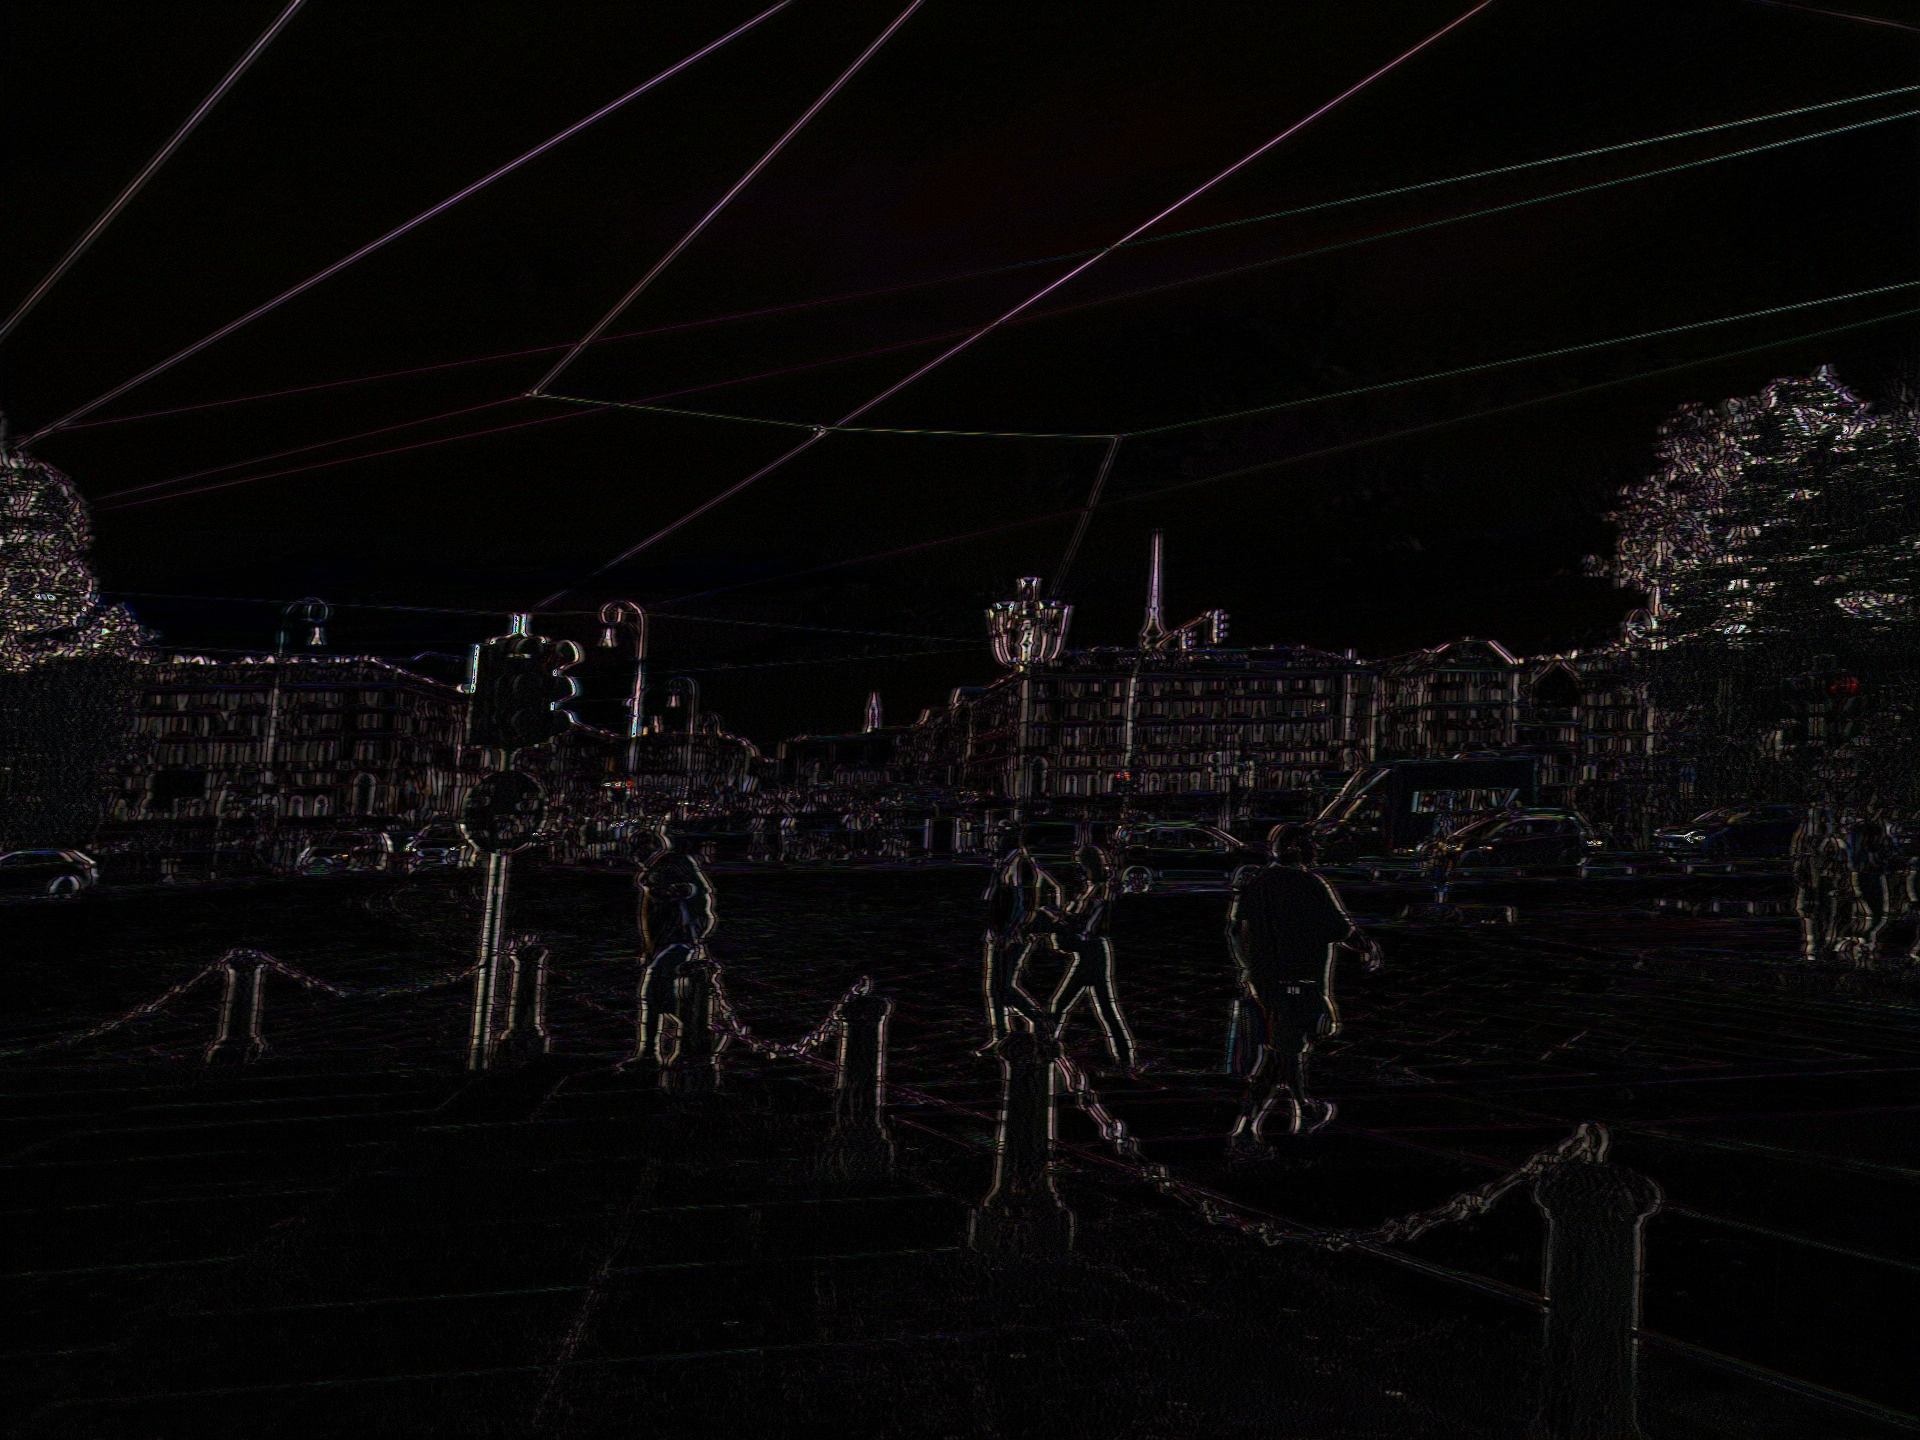
\includegraphics[width=0.31\linewidth]{figures/sample_imgs/comparison_20250503_185104.jpg}
    }\hspace{0.1cm}\hfill
    \\
    \subfloat[boh]{
      \centering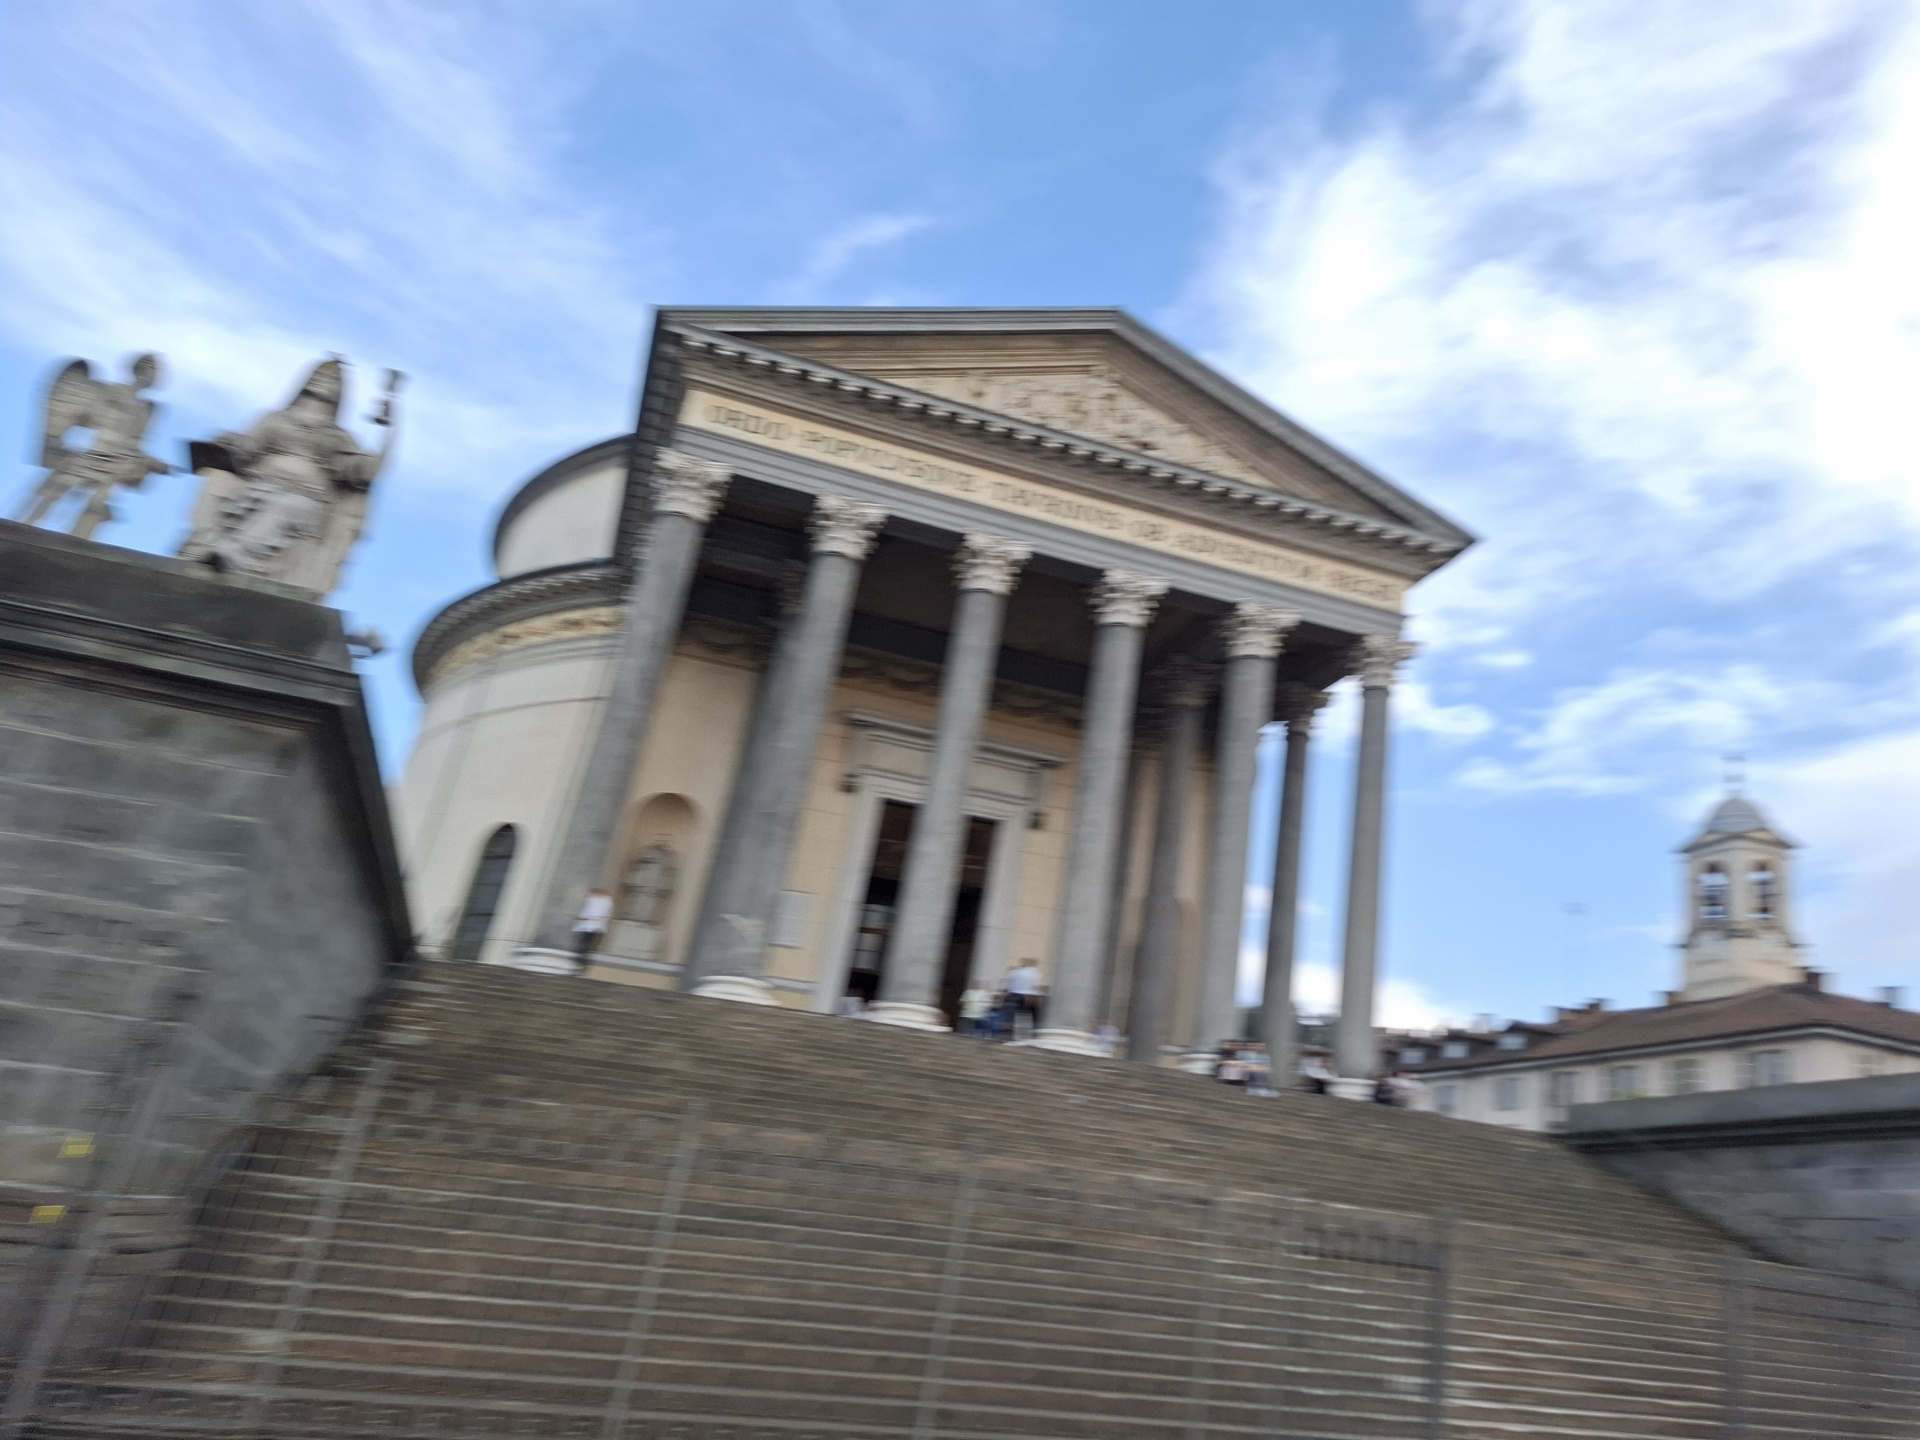
\includegraphics[width=0.31\linewidth]{figures/sample_imgs/20250503_185233.jpg}
    }\hspace{0.1cm}\hfill
    \subfloat[boh]{
      \centering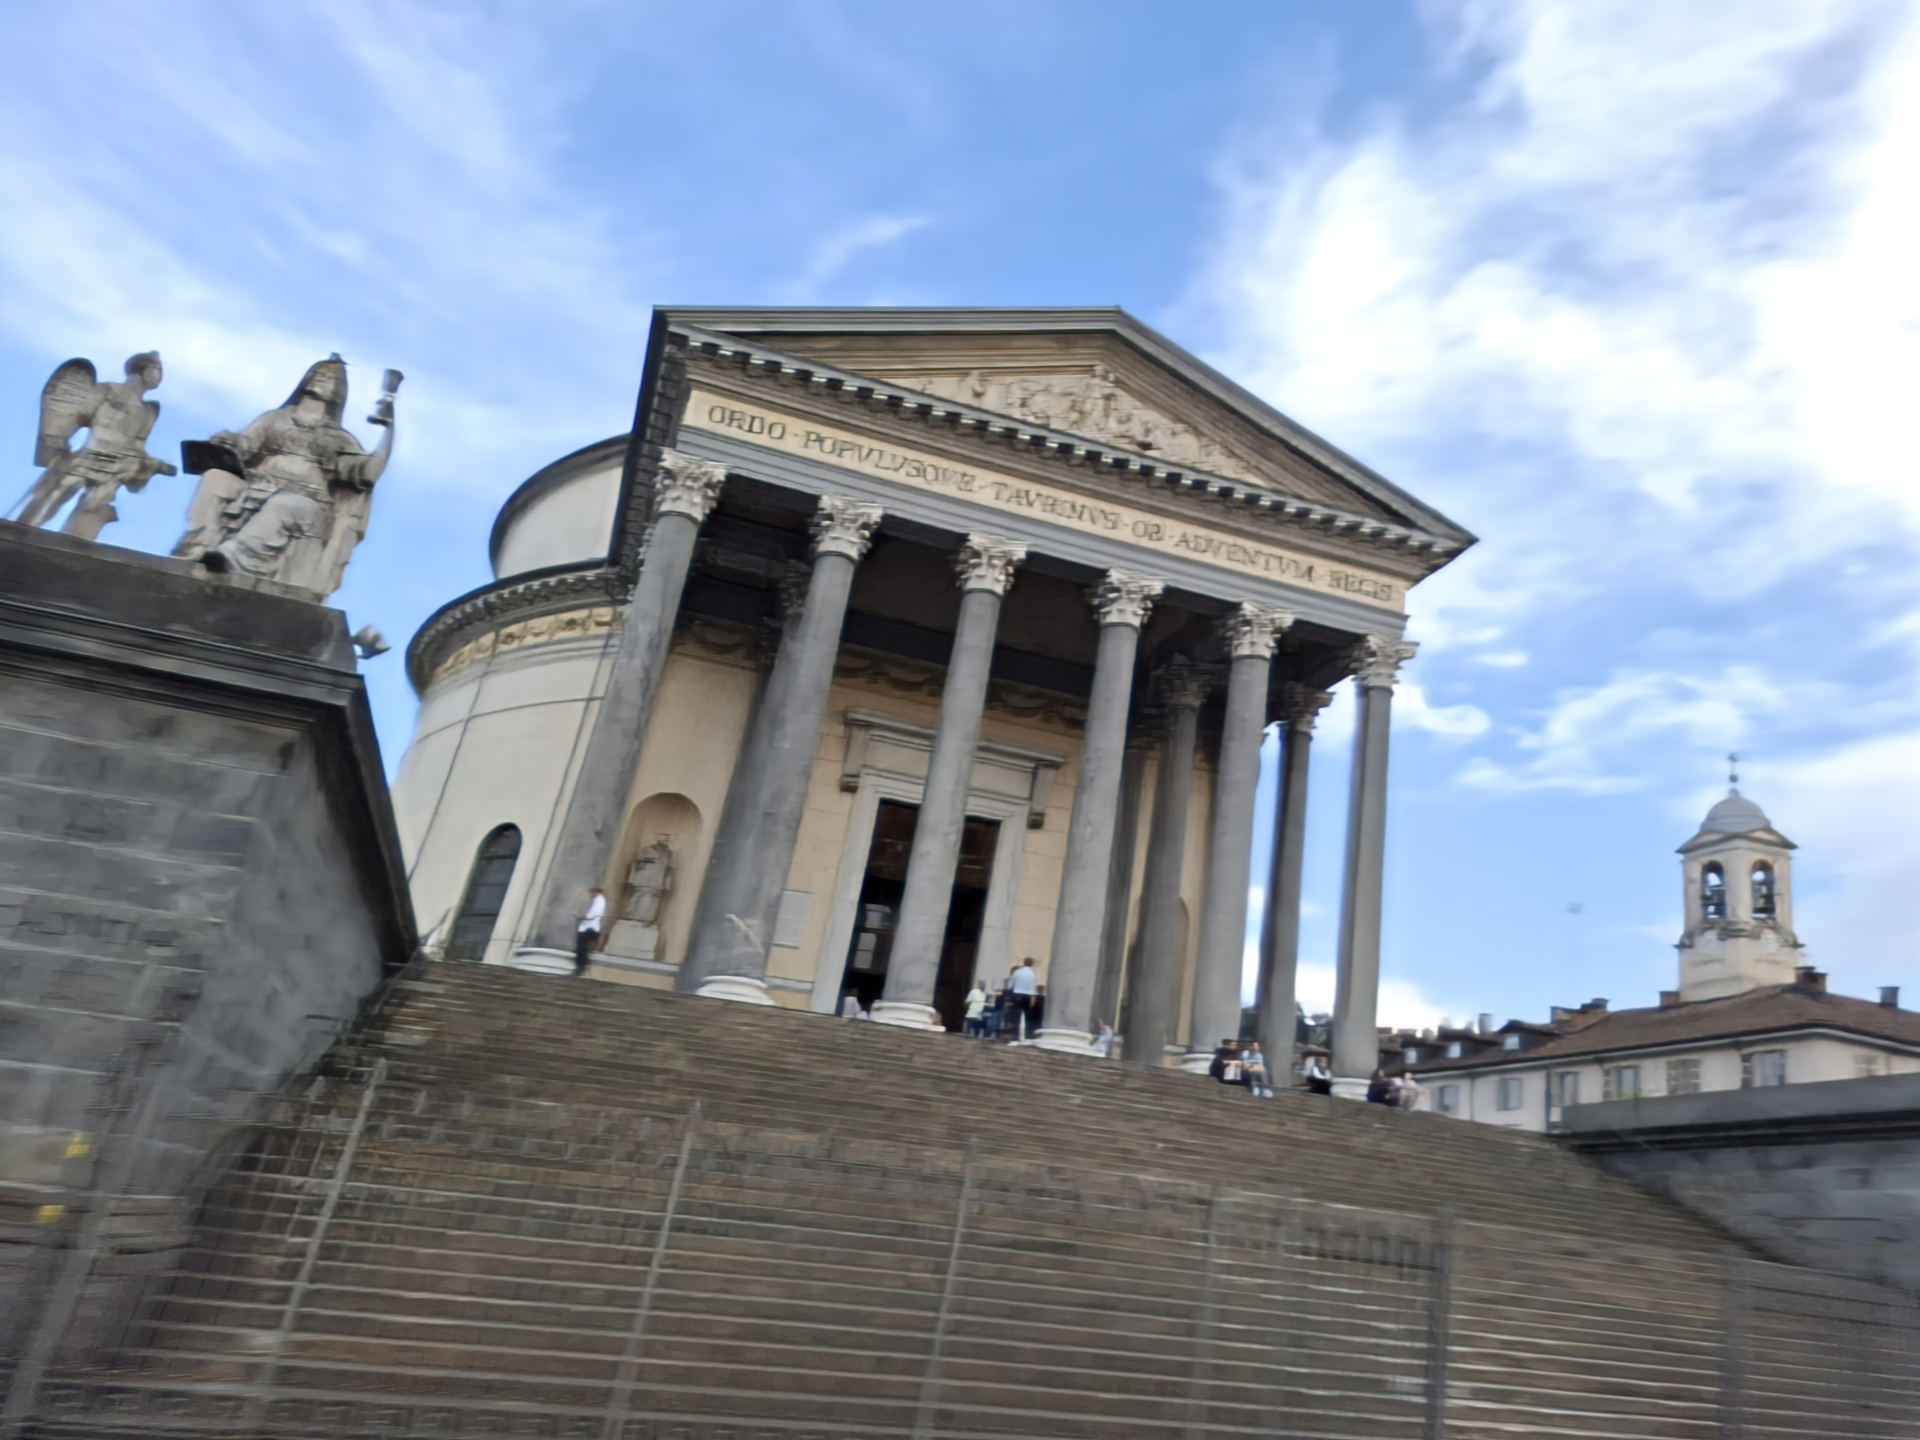
\includegraphics[width=0.31\linewidth]{figures/sample_imgs/20250503_185233_deblurred.jpg}
    }\hspace{0.1cm}\hfill
    \subfloat[boh]{
      \centering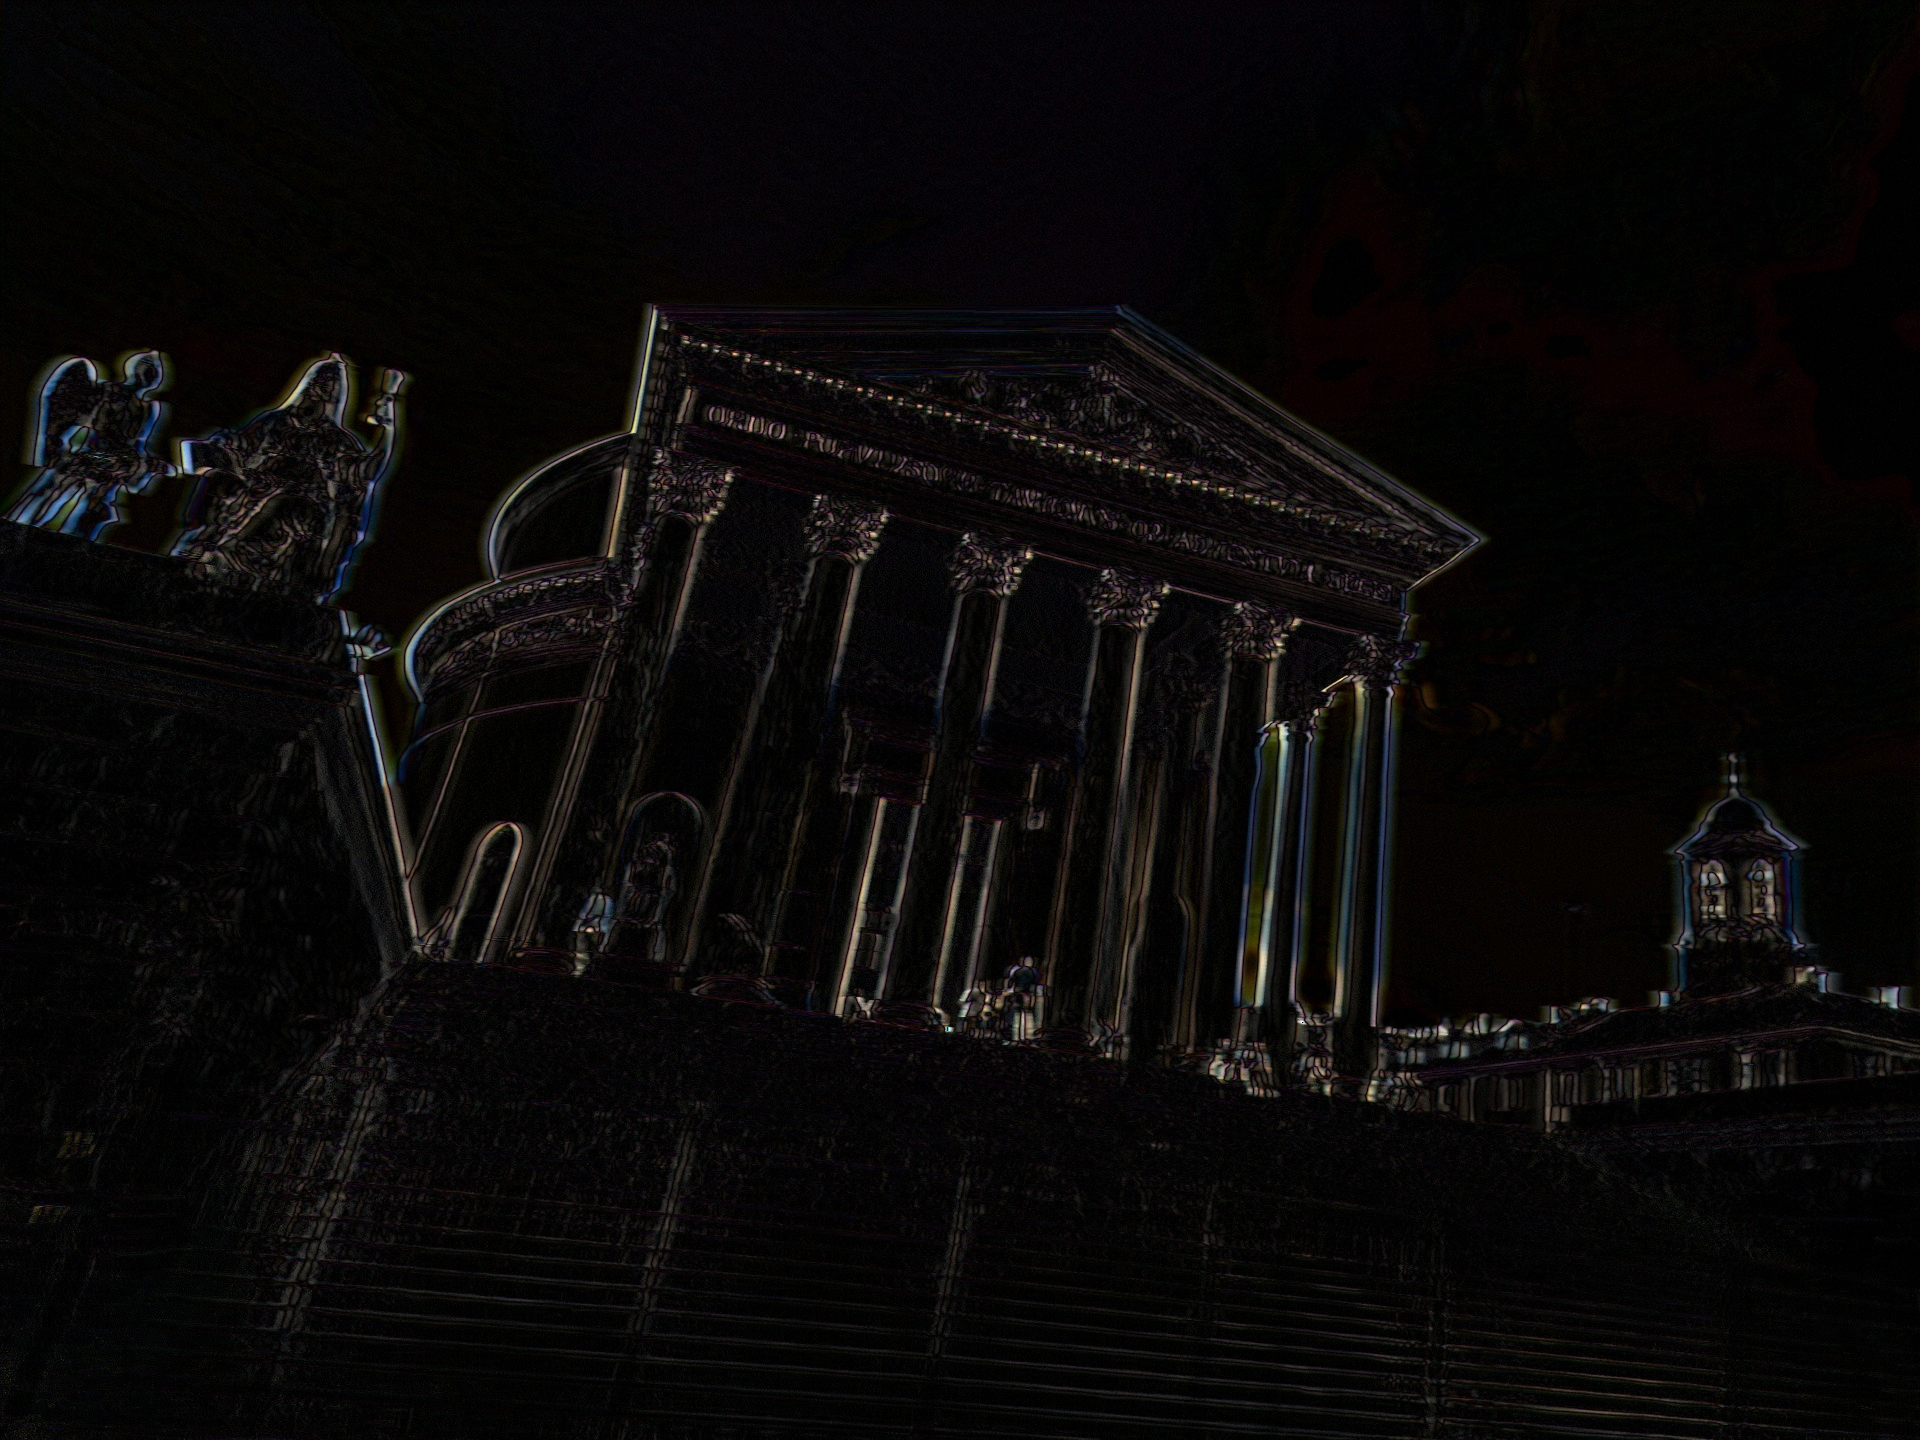
\includegraphics[width=0.31\linewidth]{figures/sample_imgs/comparison_20250503_185233.jpg}
    }\hspace{0.1cm}\hfill
    \\

    \vspace{3pt}
    \hrule
    \vspace{3pt}
    \caption{roba}
  \end{mdframed}
  \label{foto_esempio}
\end{figure*}

\FloatBarrier

\printglossary[title=Glossary, toctitle=Glossary]

\printbibliography

\end{document}

% \begin{figure}[h]\begin{mdframed}[
%       linewidth=1pt,
%       innertopmargin=6pt,
%       innerbottommargin=6pt,
%       innerleftmargin=6pt,
%       innerrightmargin=6pt
%       linecolor=black,
%       nobreak
%       ]
%     insertgraphics qua
%     \vspace{3pt}
%     \hrule
%     \vspace{3pt}
%     \caption{}
% \end{mdframed}\end{figure}
